\chapter{The Calorimeter Layer-1 Trigger Primitives calibration}

\section{A novel Machine Learning method for detector objects calibration}
\label{sec:A novel Machine Learning method for detector objects calibration}

The energy calibration of calorimeters at collider experiments is of paramount importance for the physics performance.
Calorimeters are designed to measure the energy of high energy particles, such as photons and electrons producing electromagnetic showers, or quarks generating the hadronic showers due to color confinement and hadronisation. Whether it is a homogeneous calorimeter, capable of absorbing the energy of the particle shower in its entire depth, or a sampling calorimeter, where the energy is only detected in the active layers alternated to passive absorbers, calorimeters are hardly able to provide uniform response across the whole spatial and energy range. Calibration procedures are therefore fundamental to ensuring accurate energy measurement.

In order to improve spatial resolution in the reconstruction of the particles position, calorimeters can be segmented in the longitudinal and transverse directions, into ``calorimeter cells''. 
By clustering multiple cells together, it is possible to reconstruct the full shower energy deposit, whilst the spatial sampling can provide information about the particle position and, based on that, infer its four-momentum.
The essence of energy calibration consists of determining the optimal coefficients, known as calibration constants, that correct the individual cells energy, such that the energy of reconstructed particles aligns as closely as possible with their true energy. 
Several approaches exist to calibrate calorimeter cells.
For instance, in the case of the CMS electromagnetic calorimeter (ECAL), calibration constants are derived by either laser monitoring, i.e. using a laser a standard source of light to induce a response in the ECAL cells (lead-tungsten scintillating crystals), or by physics events such as photons from $\pi^0$ or $\eta$ meson decays, or electrons from $W$ or $Z$-boson decays~\cite{Cavallari:2798128}. These methods provide essential insights into the response of calorimeter cells, ensuring accurate energy reconstructions, crucial for precise particle physics measurements.

This chapter explores a novel machine learning approach tailored to effectively calibrate calorimeter objects by using higher-level and better-calibrated physics objects as a reference, such as the offline reconstructed particle energy.
The main advantage of the method is the possibility of calibrating CMS sub-detectors directly using data from proton-proton collisions or from test beams. This possibility is particularly beneficial when Monte Carlo simulations are not entirely reliable or not available.
Moreover, the method is particularly convenient when the number of cells is extremely high, such as for the future High Granularity Calorimeter (HGCAL), due to the scalability of ML methods and to the capabilities in treating and learning from a large number of input data simultaneously.

A proof of concept of the method has been implemented in the context of the Layer-1 Calorimeter Trigger Primitives calibration, where the number of parameters and the complexity of the trigger information are reduced. However, the performance of the method provides an improvement in the energy resolution that can be highly beneficial for the L1 Trigger efficiency.

% The technique uses Machine Learning to derive a set of calibration constants, optimized such that the sum of the calibrated cells energy approaches the energy of the corresponding reference object. In particular, I have played a major role in the first application of this technique, which was the calibration of the calorimeter trigger tower at Level-1 Trigger. In this context, the calibration constants depend on the trigger tower raw energy and position, and the algorithm targets the energy of the matched offline reconstructed electron or jet. We implemented the optimization algorithm using differentiable programming with the JAX Python library, which allows for the definition of custom losses and a fully configurable minimization. As one of the main project developers, I have also actively contributed to the the simulation and study of the input data, the hyperparameter optimization and the performance evaluation on electron and jet datasets. The corresponding set of scale factors will soon be deployed online. It is expected that the technique will also be employed in other contexts going forward, for example in the calibration of HGCAL cells."


\section{The calibration method applied to the Level-1 trigger}
\label{sec:The calibration method applied to the Level-1 trigger}

The CMS L1 Trigger system provides an optimal playground for testing the novel calibration approach, with the aim of improving the energy resolution of the trigger objects and providing a more efficient event selection.
The function of the L1 Trigger consists in combining the data coming from the CMS sub-detectors, detecting the potential presence of high energy objects or other interesting event features, to decide whether to accept or discard a given collision event. The role of the L1 Trigger system is essential to reduce the LHC collision rate of 40~MHz to only 100~kHz, the maximum data streaming rate reachable by the CMS data taking system.
The decision-making needs to occur within the 3.8~$\mu$s available latency, for this reason, the L1 decision cannot be based on the full event information, but on low resolution physics objects that only rely on the inputs coming from the calorimeters and the muon system, called \textit{L1 candidates}.
The input to the L1 Trigger is the so-called \textit{Trigger Primitives} (TPs), which are either produced by on-detector electronics placed in the experimental cavern, or by off-detector electronics in the service cavern. The TPs offer a coarse view of the physics event and can be combined together for the L1 object candidates. 

To operate a decision, the L1 trigger collects the information from the calorimeters and from the muon detectors separately. The object definition is run independently in the two sub-systems and combined at the final step by the Global Trigger algorithm, which performs the event accept or reject decision based on the L1 candidates kinematics and high-level variables, such as invariant masses and angular distances.

For this work, only the Calorimeter Trigger system has been considered for the application of the calibration method. In the calorimeter system, the information of the energy deposit in the HCAL and ECAL sub-detectors is processed by two consecutive systems, called respectively \textit{Layer-1} and \textit{Layer-2}. In the Layer-1 system, the TPs are calibrated and pre-processed before being sent to Layer-2 for object reconstruction. Given the stacked architecture of the two systems, better-calibrated objects at the output of the Layer-1 system can lead to significant improvement in the performance of the Layer-2 object definition, which would propagate in a more effective L1 Trigger decision.
The novel ML-based calibration method has been consequently applied to the calibration procedure of the Layer-1 calorimeter Trigger Primitives.
% One important example of how a lower- level calibration can largely benefit high-level objects is the PF algorithm; in this approach, the proper calibration of the PF elements ensures that the final PF candidates are well calibrated, and their high-level calibration factors are generally close to unity. For this reason, as part of this Thesis work, I have been the leading contributor to developing a novel technique for calibrating calorimeter TPs. This method is based on a ML approach and exploits offline reconstructed electrons and jets to calibrate single TPs optimally. This ML technique is detailed in the present Section; first, a brief overview of the past approach to TP calibration is given, highlighting its critical points, then the new method is described in detail, followed by the presentation of its performance.

\subsection{The Layer-1 calorimeter inputs}
\label{subsec:The Layer-1 calorimeter inputs}

The information from the ECAL, HCAL, and Hadron Forward (HF) detectors are transmitted to the L1 trigger system in the form of TPs, which are digital quantities corresponding to the 40~MHz samplings of the calorimeter pulses. Each sub-detector TP reflects the localised energy deposit in a specific sub-detector region, corresponding to an extension of $\Delta\eta\times\Delta\phi = 0.087 \times 0.087$ in the barrel: for ECAL each TP covers a square of $5\times5$ grid of crystals, while for HCAL it is equivalent to a single read-out unit.
Each half barrel of the CMS detector is consequently divided into 17 TPs along the $\eta$ direction, and into 72 TPs along the $\phi$ direction. Therefore, a discrete Trigger Tower two-indices Cartesian notation is employed to identify each TP using the pair ($i\eta$, $i\phi$). In this configuration, the TPs in the barrel have $i\eta$ and $i\phi$ indices such that $i\eta \in [-17,17] \setminus \{0\}$ and $i\phi \in [1,72]$, excluding position 0 from both directions.

A more complex definition of the TPs is required for the endcaps and HF, due to the varied geometry of the detector components.
In the ECAL endcap, where crystals are arranged in the specific pattern represented in Figure~\ref{fig:EE_HF_L1TP}~(a), to allow for a detailed analysis of the lateral energy spread of electromagnetic showers. In this region, the TPs do not follow exact ($\eta$, $\phi$) boundaries, but are defined in such a way that their extension in the $\eta$ dimension decreases radially as they approach the beam pipe. The resulting number of crystals in each TP varies from 25 for $|\eta|\sim1.5$ to 10 for $|\eta|\sim2.8$. 
This geometry is mainly designed to align with the HCAL tower geometry while maintaining a uniform segmentation of the detector.
In the HCAL endcap, each physical tower, which has an extension of $\Delta\phi = 0.174$, is evenly split into two TPs of $\Delta\phi = 0.087$. 
In this setup, the TPs in the endcap have $i\eta$ and $i\phi$ indices such that $|i\eta| \in [18,28]$ and $i\phi \in [1,72]$. 

For the HF detector, the same $\phi$-splitting geometry as the HCAL endcap is used, while the $\eta$ direction is divided into 12 segments, giving $|i\eta| \in [29,41]$ and $i\phi \in [1,72]$, as illustrated in Figure~\ref{fig:EE_HF_L1TP}~(b).

The CMS calorimeter trigger system has a total of 4,176 towers distributed in: 
\begin{itemize}
    \item 2,448 TPs in the ECAL and HCAL barrel,
    \item 1,584 in the ECAL and HCAL endcap,
    \item 144 in the HF calorimeter.
\end{itemize}
Figure~\ref{fig:Layer1} provides a schematic representation of the TP geometry. 

\begin{figure}
    \centering
    \subfloat[]{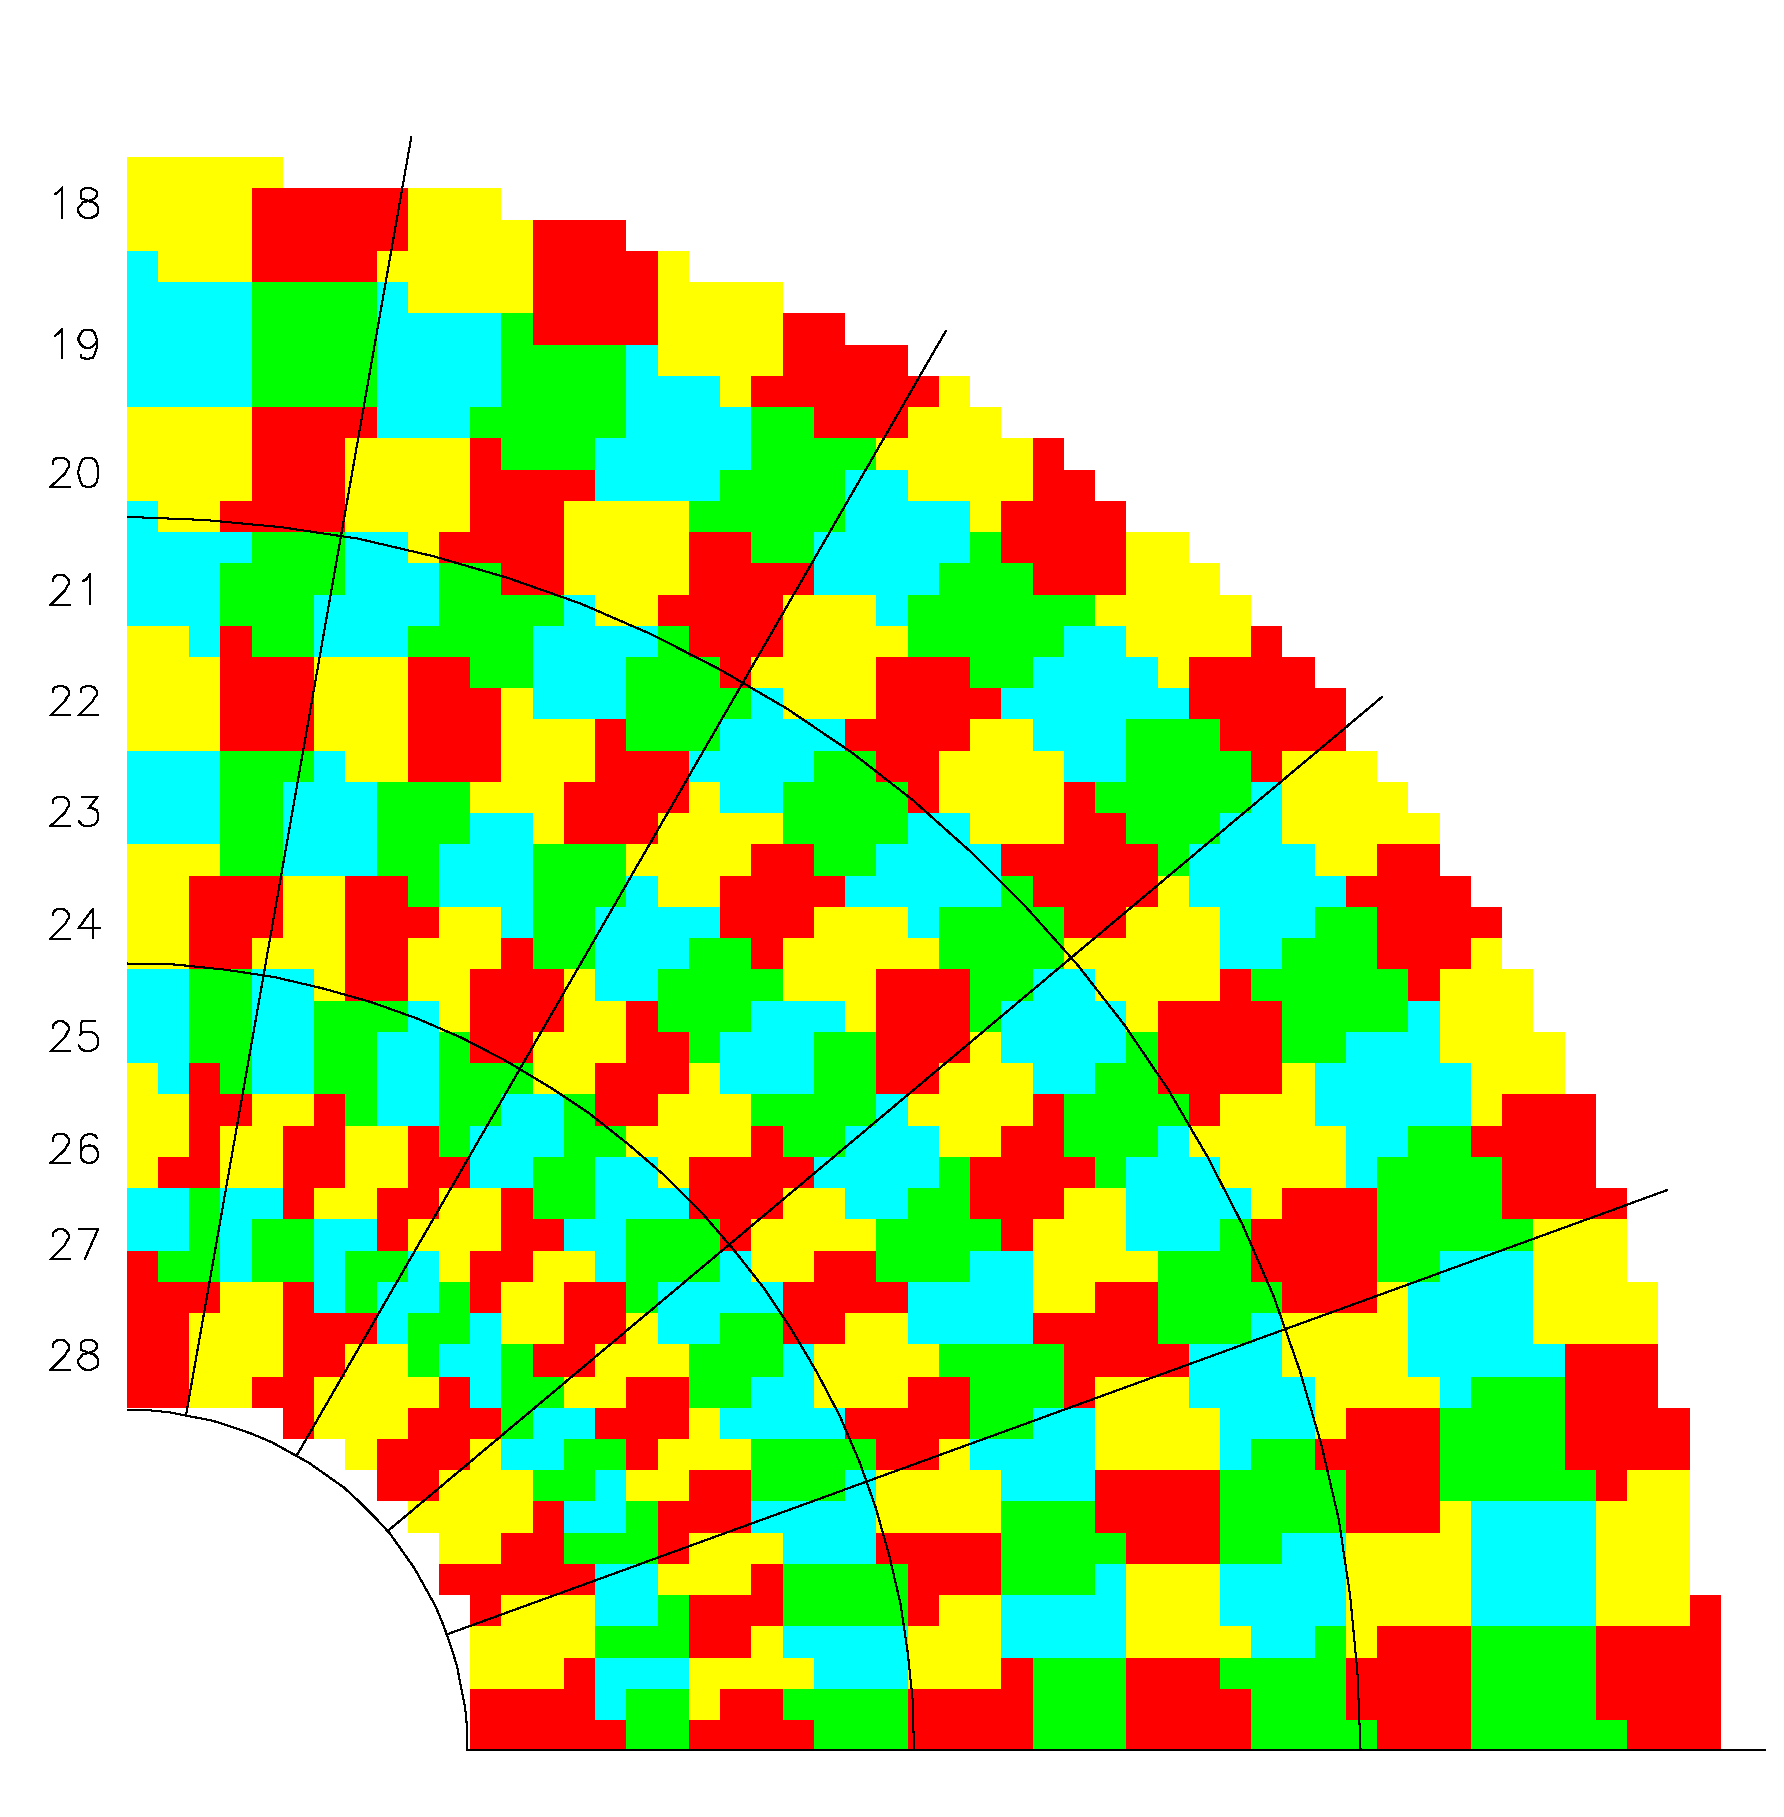
\includegraphics[width=0.4\linewidth]{Figures/L1TP/EE_L1TP.pdf}}
    \subfloat[]{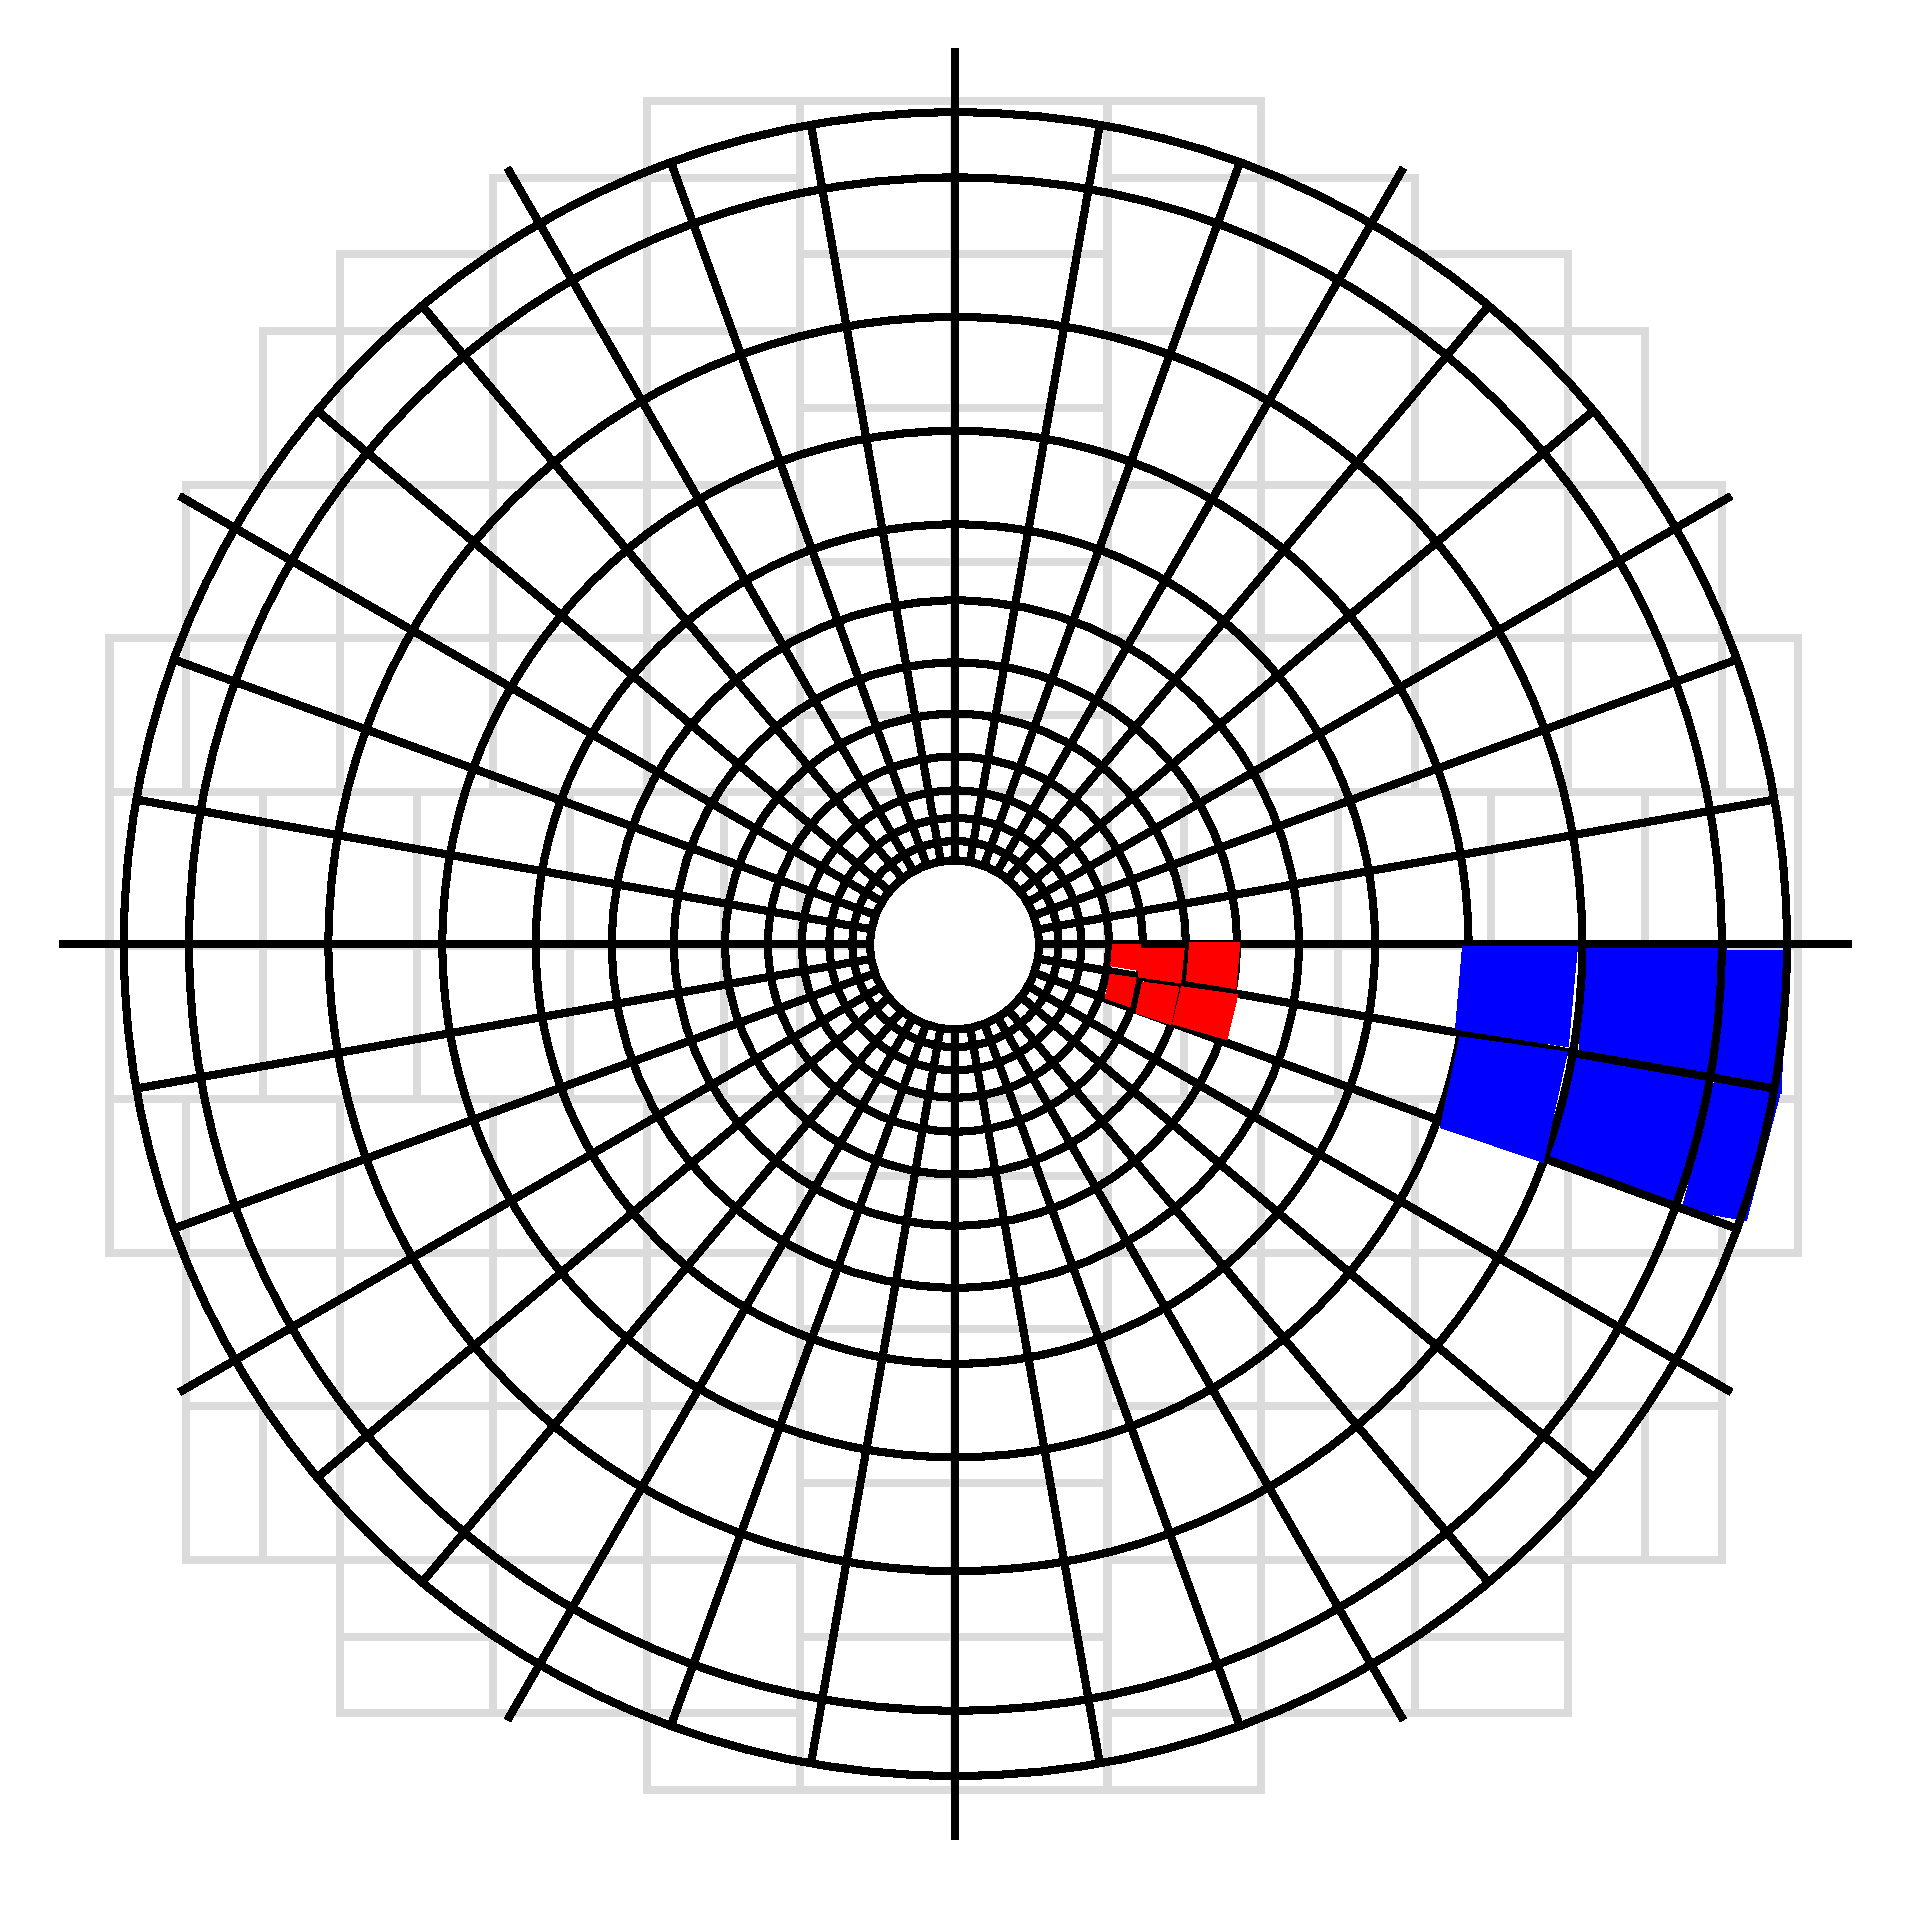
\includegraphics[width=0.4\linewidth]{Figures/L1TP/HF_L1TP.pdf}}
    \caption{Calorimeter Trigger Primitives (TP) layout in the x–y projection of the ECAL endcap (a); each square denotes a different ECAL crystal, and regions characterised by the same color represent one TP.
    Calorimeter TPs layout in the x–y projection of the HF detector (b); each square denotes a HF read-out unit, and regions with the same colour represent one Trigger Tower (TT).}
    \label{fig:EE_HF_L1TP}
\end{figure}

\begin{figure}
    \centering
    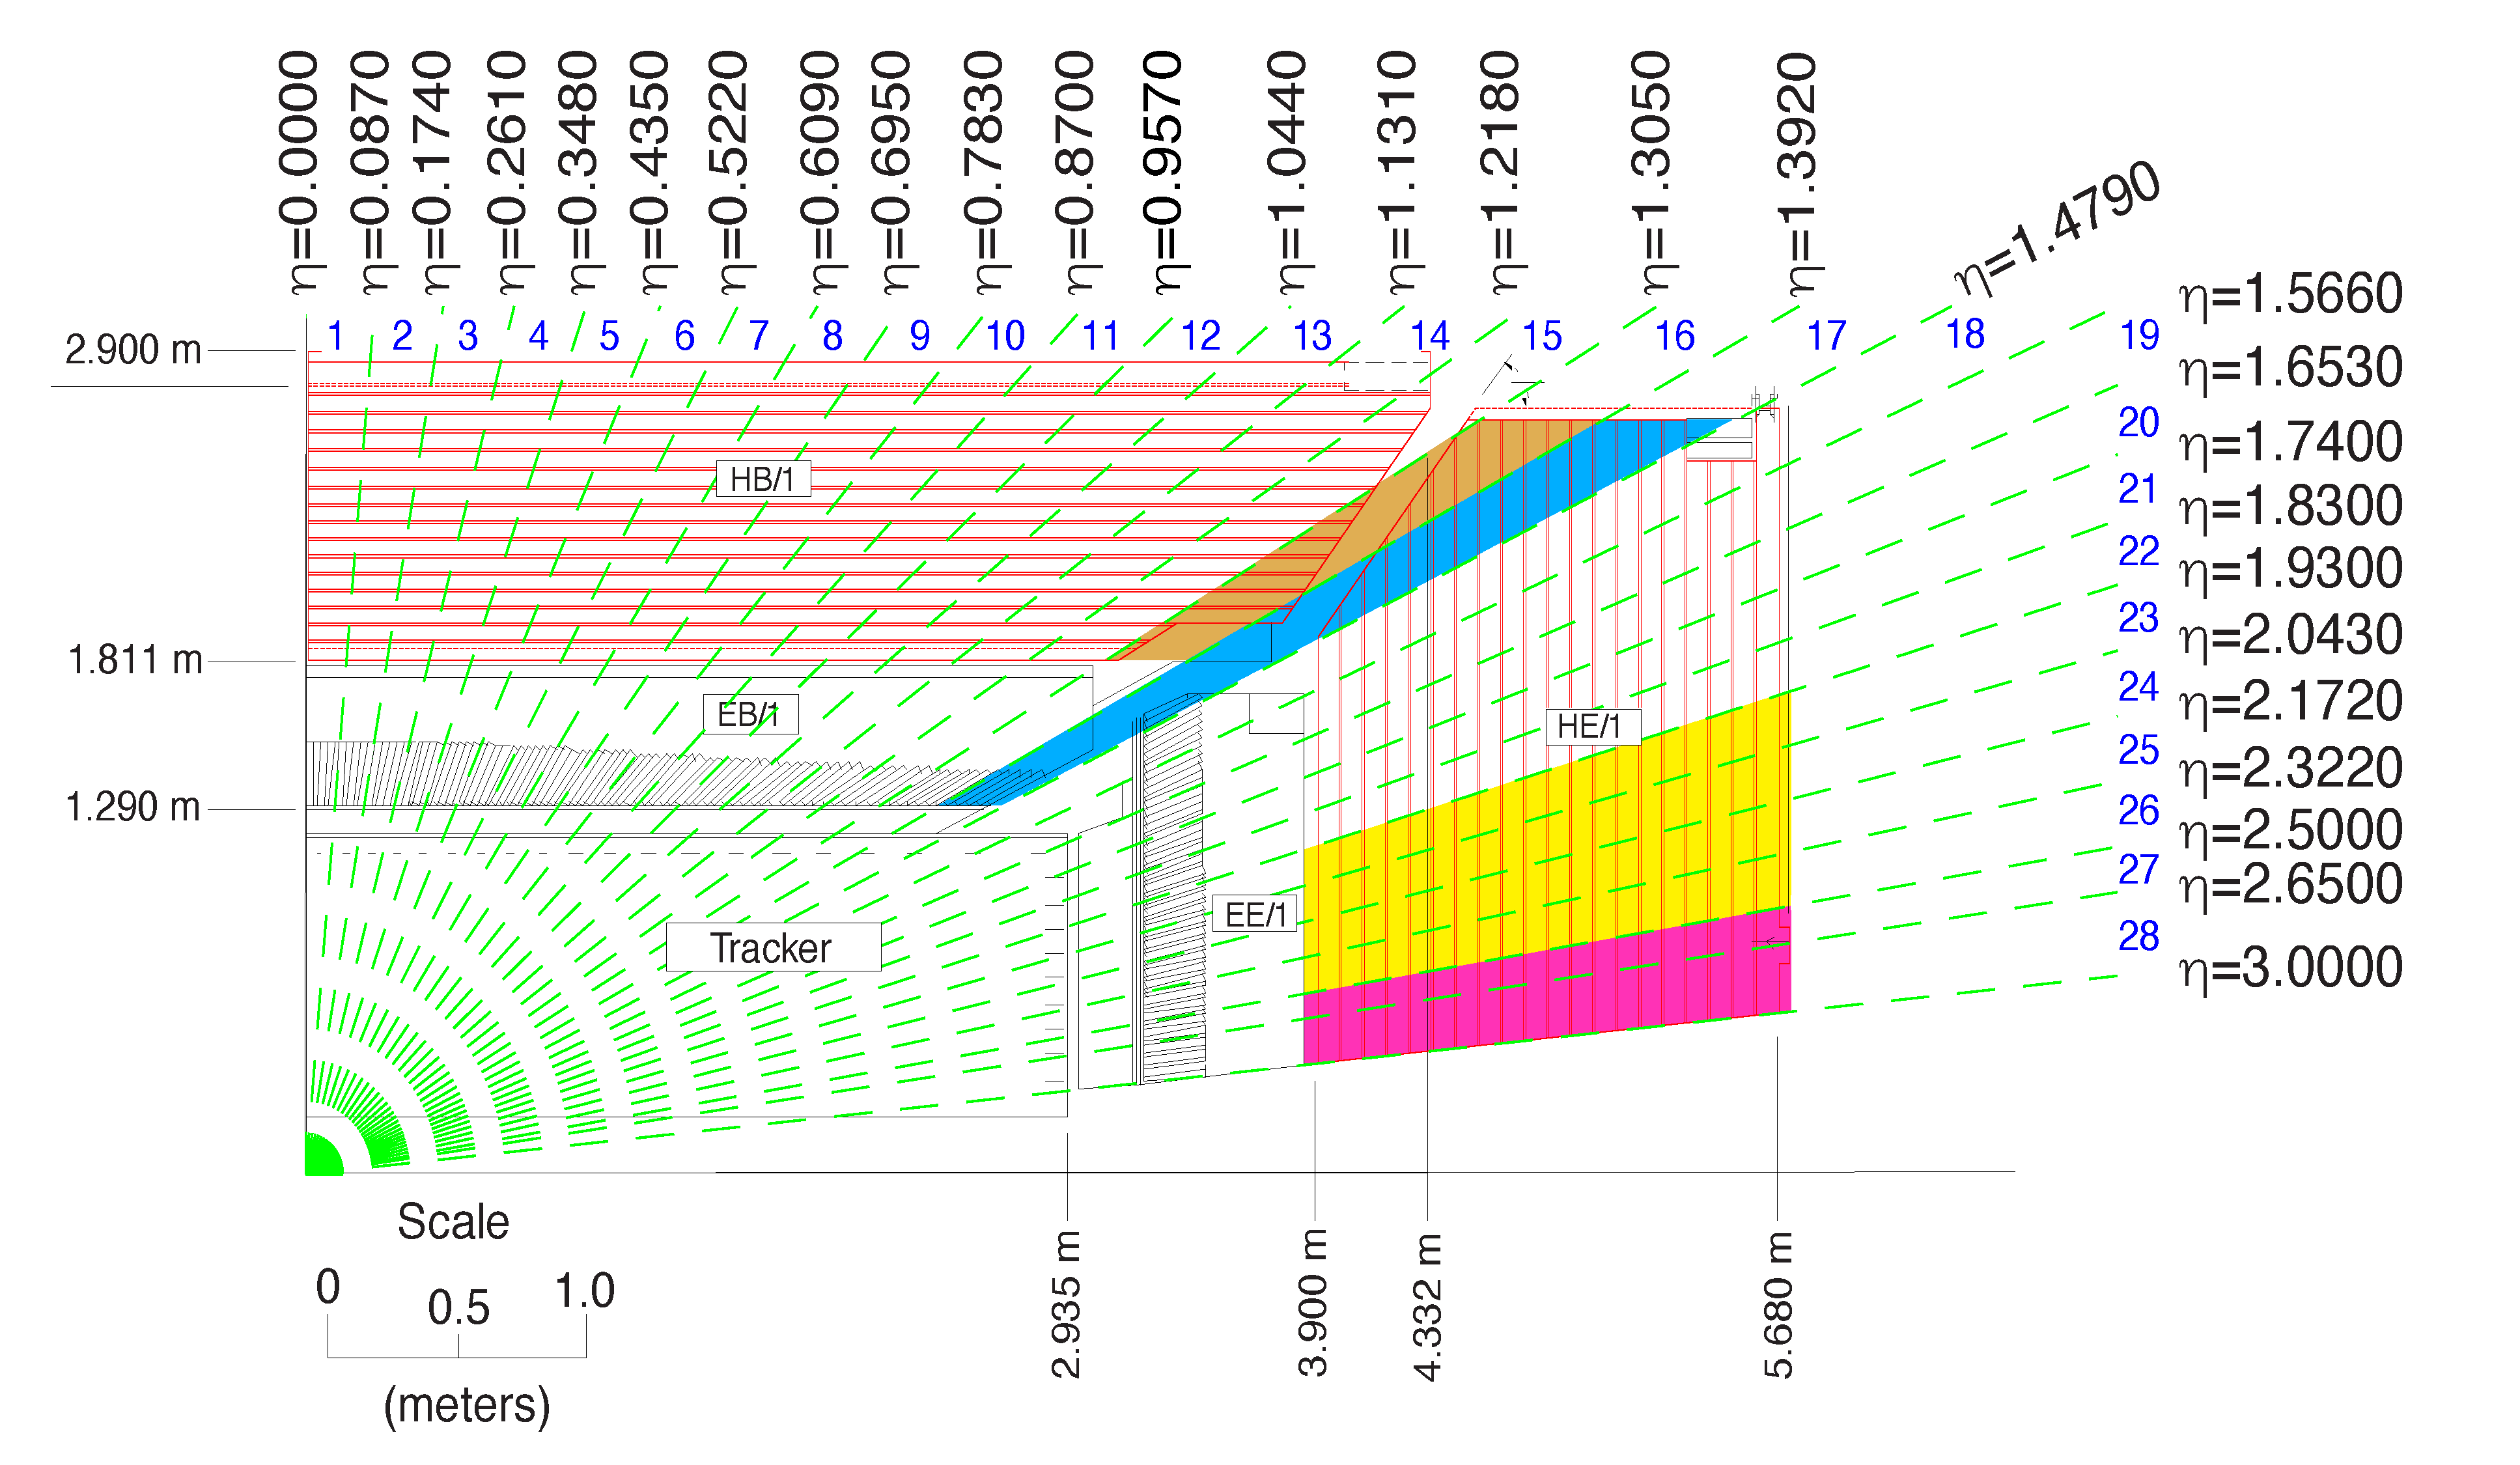
\includegraphics[width=0.9\linewidth]{Figures/L1TP/L1TP.pdf}
    \caption{Schematic view of the ECAL and HCAL TP separation in the $r$-$z$ projection of the CMS detector. }
    \label{fig:Layer1}
\end{figure}

\bigbreak

Each TP is characterised by a ($i\eta$, $i\phi$) position and a transverse energy, denoted as $E_T$.
The energy deposit is computed as the projection onto the transverse plane of the momentum vector originating in the detector centre and pointing to the calorimeter cells. This value is encoded into 8-bit digital quantities, corresponding to 256 possible values: each bit correspond to a 0.5~GeV unit, therefore each TP can transmit up to 127.5~GeV and higher values are saturated to the maximum.
The ($i\eta$, $i\phi$) position, instead, does not need to be encoded into digital quantities as it is fully determined by the linking in the detector read-out to the calorimeter trigger Layer-1.

The ECAL and HCAL TPs are transmitted to the Layer-1 calorimeter trigger, where a calibration factor is applied to each of them, based on position and energy deposit. Beside correcting for the detector non-homogeneity, the Layer-1 calibration can adjust the inter-calibration between the energy recorder in ECAL and HCAL TPs.
After the calibration, the ECAL and HCAL TPs that geometrically lie one behind the other are combined together into Trigger Towers (TTs).
A particular configuration is followed for the HF detector, where coarser TT granularity is adopted, with a segmentation of 4 TTs in $\eta$ and of 18 TTs in $\phi$ direction. 
Each TT is characterised by a 16-bit digital quantity that encodes a 9-bit word reporting the total $E_T$ from both ECAL and HCAL, the ratio of the ECAL and HCAL energies on 5 bits, and HCAL and ECAL quality flags on the 2 remaining bits.
At this stage, TTs can contain up to 255~GeV, and any TT with $E_T \geq 0.5$~GeV is referred to as an \textit{fired tower}. 
Finally, the Layer-1 sorts the TTs in descending $E_T$ order and transmits them to Layer-2, where any of the Master Processor (MP7) cards receives the complete set of TTs from each bunch crossing. 

\subsection{The Layer-2 calorimeter objects}
\label{subsec:The Layer-2 calorimeter objects}

In the Layer-2 calorimeter trigger, the TTs are merged together to form L1 objects. The L1 reconstruction algorithms have been developed and optimised to reconstruct electrons, photons, jets, hadronically decaying tau leptons, and energy sums.
Such algorithms need to access the full calorimeter information and require fast computing power furnished by Field-Programmable Gate Arrays (FPGAs) firmware.
A brief overview of the L1 calorimeter candidates reconstruction algorithms is given in the following paragraphs.

\subsubsection{Electrons and photon candidates}

Due to the unavailability of the tracking information at the L1 stage, electrons and photons are indistinguishable and grouped together in the $e/\gamma$ category, or \texttt{EGamma}.
The L1 $e/\gamma$ candidate is initiated by the presence of a high energy deposit in a single TT, also called \textit{seed}. The TTs around the seed are dynamically clustered~\cite{Sauvan_2015} to the seed according to their position and recorded energy.
The maximum cluster size is limited to 8 TTs, in order to minimise the impact of pile-up energy deposits while including most of the electron or photon energy.
Since electron and photon showers spread mostly along the $\phi$ direction due to the CMS magnetic field, an extended region in $\phi$ (5 TTs at most) and narrow in $\eta$ (2 TTs at most) is chosen.
The first and second neighbour fired TTs are clustered only if connected to the seed, as shown in Figure~\ref{fig:L1EGammaCluster}~(left).
The dynamic clustering leads to a large variety of cluster shapes depending on the distribution of the energy around the seed tower. Large clusters involving many trigger towers are probably produced by the pre-showering of jets in ECAL, while small clusters, containing typically one to four TTs, are more compatible with electron or photon showers. For this reason, the shape of the cluster, which would not be available for a fixed size clustering, is an important information for the particle candidate and brings additional discrimination power between electrons (or photons) and jets.

The sum of the ECAL $E_T$ of the seed and clustered towers is considered the raw $E_T$ of the $e/\gamma$ cluster, which is calibrated using Layer-2 scale factors dependent on the $\eta$-position of the seed tower. These calibration factors, derived from $Z \rightarrow ee$ events, are defined as the ratio of the offline reconstructed electron $E_T$ to the corresponding raw L1 cluster $E_T$.
Since the Layer-2 calorimeter trigger has access to TTs without boundaries, it is possible to account for the pile-up conditions by applying isolation requirements. The isolation energy is computed in a $5\time9$ TTs region, excluding the $e/\gamma$ candidate footprint in ECAL ($2\times5$ TTs) and HCAL ($1\times2$ TTs). The isolation region is better illustrated in Figure~\ref{fig:L1EGammaCluster}~(right). The isolation threshold depends on the $i\eta$ position of the cluster and on an estimator for the number of pile-up interactions, given by the number of TTs in the whole detector acceptance recording an energy $E_T>4$~GeV. 
Finally, an energy-dependent threshold on the ration between ECAL and HCAL energy deposit, also known as $E/H$, is applied to reduce the mis-identification rate of hadronic showers.

\begin{figure}
    \centering
    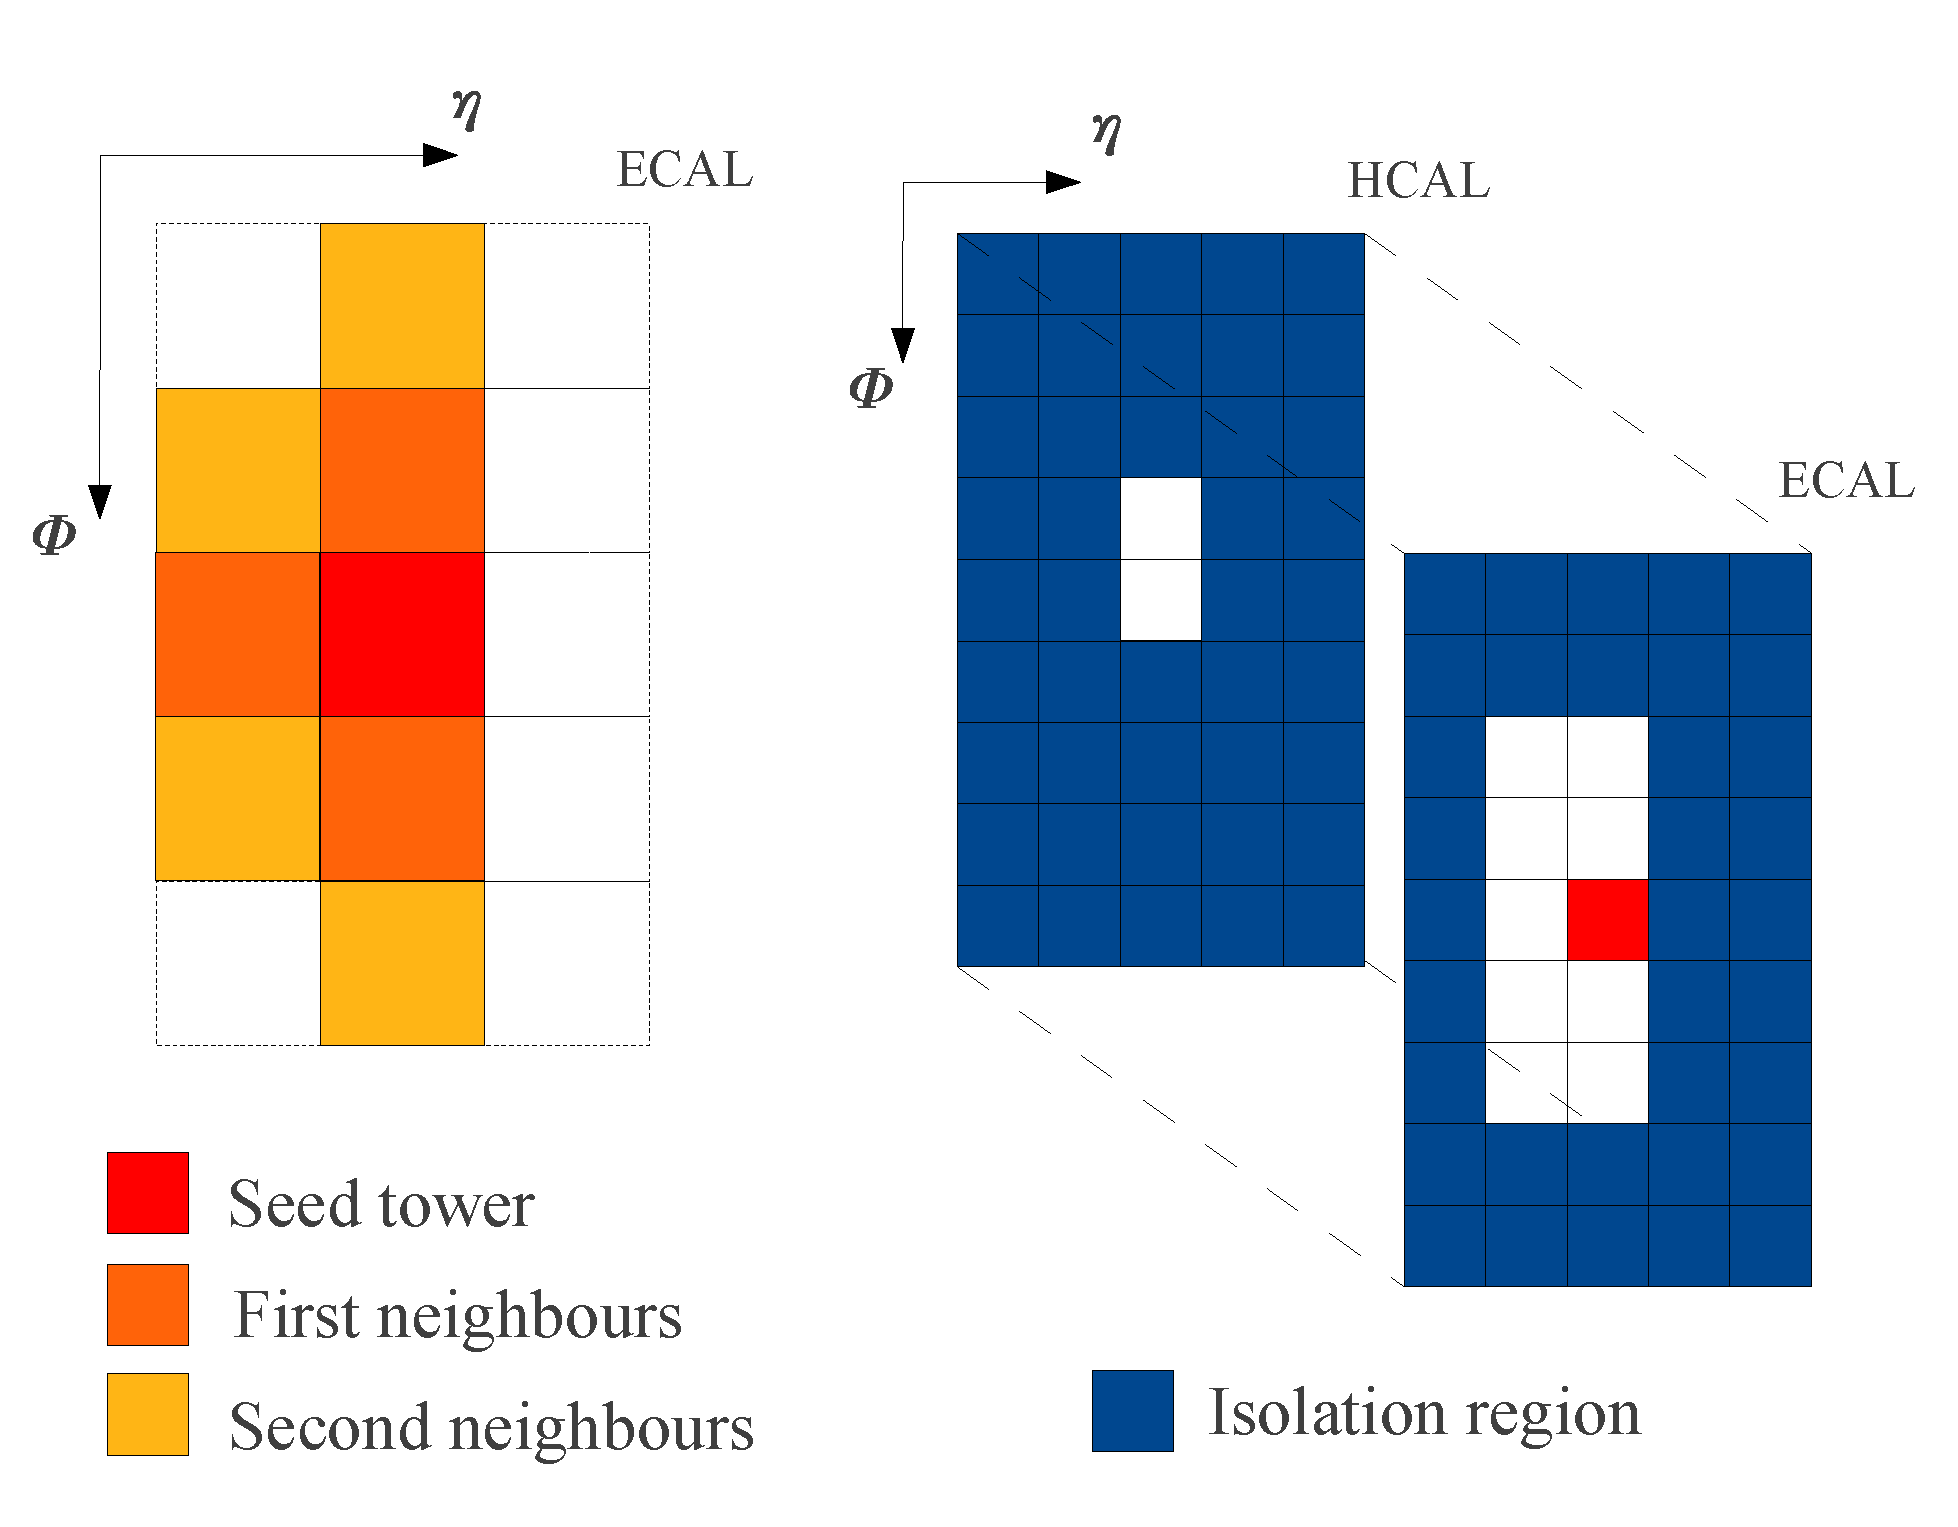
\includegraphics[width=0.5\linewidth]{Figures/L1TP/L1EGammaCluster.pdf}
    \caption{Schematic for the L1 $e/\gamma$ dynamic clustering and isolation. A candidate is formed by clustering around the seed all the fired neighbour towers. A candidate is considered as isolated if the $E_T$ in the ECAL and HCAL isolation regions is smaller than a given value.}
    \label{fig:L1EGammaCluster}
\end{figure}

\subsubsection{Hadronic tau lepton candidates}

Hadronically decaying $\tau$ leptons are reconstructed by the Layer-2 calorimeter trigger with an algorithm similar to the one used for $e/\gamma$ candidates.
The most probable products for the tau leptons hadronic decay are pions, which can leave energy deposit both in the ECAL and the HCAL calorimeters. 
The $\tau_h$ candidate selection begins a single TT seed, and the TTs around the seed, in a region spanning 5 and 9 TTs in the $\eta$ and $\phi$ directions respectively, are merged following the dynamic cluster procedure.
The TTs within one unit in $i\eta$ and $i\phi$ from the seed, and the ones on the same $i\eta$ position at two units distance in $i\phi$, are incorporated into the \textit{proto-cluster}. A subsequent \textit{lateral trimming} procedure is implemented to remove the least energetic side of the proto-cluster, as shown in Figure~\ref{fig:L1TauCluster}~(left).

Since the $\tau_h$ decay can produce several charged or neutral pions, leading to broader energy deposit. 
For this reason, at the same as the primary proto-cluster creation, \textit{secondary clusters} are built with the same approach, but considering a smaller window spanning 3 TTs in both $\eta$ and $\phi$ directions.
The secondary clusters are merged to the primary proto-cluster only if their seed is found in one of the eight positions highlighted in green in Figure~\ref{fig:L1TauCluster}~(right). An overlap procedure is applied to avoid double-counting of TTs in multiple clusters.
The sum of all the TTs $E_T$ included in the merged cluster is considered to be the raw $E_T$ of the $\tau_h$ cluster, which is calibrated using Layer-2 scale factors dependent on raw energy deposit, the $\eta$-position of the seed tower, the presence of ECAL energy deposit, and the cluster being issued by the merging procedure or not.
Also for $\tau_h$ candidates, an isolation requirement is applied to reduce contamination from hadronic jets, characterised by wider calorimeter activity. The isolation energy is computed in a $6\time9$ TTs region, excluding the $\tau_h$ candidate footprint.
The isolation threshold depends on the raw energy deposit, on the $i\eta$ position of the cluster, and on an estimator for the number of pile-up interactions, given by the number of fired TTs in the most central region of the barrel, i.e. $|i\eta|\leq 4$.

\begin{figure}
    \centering
    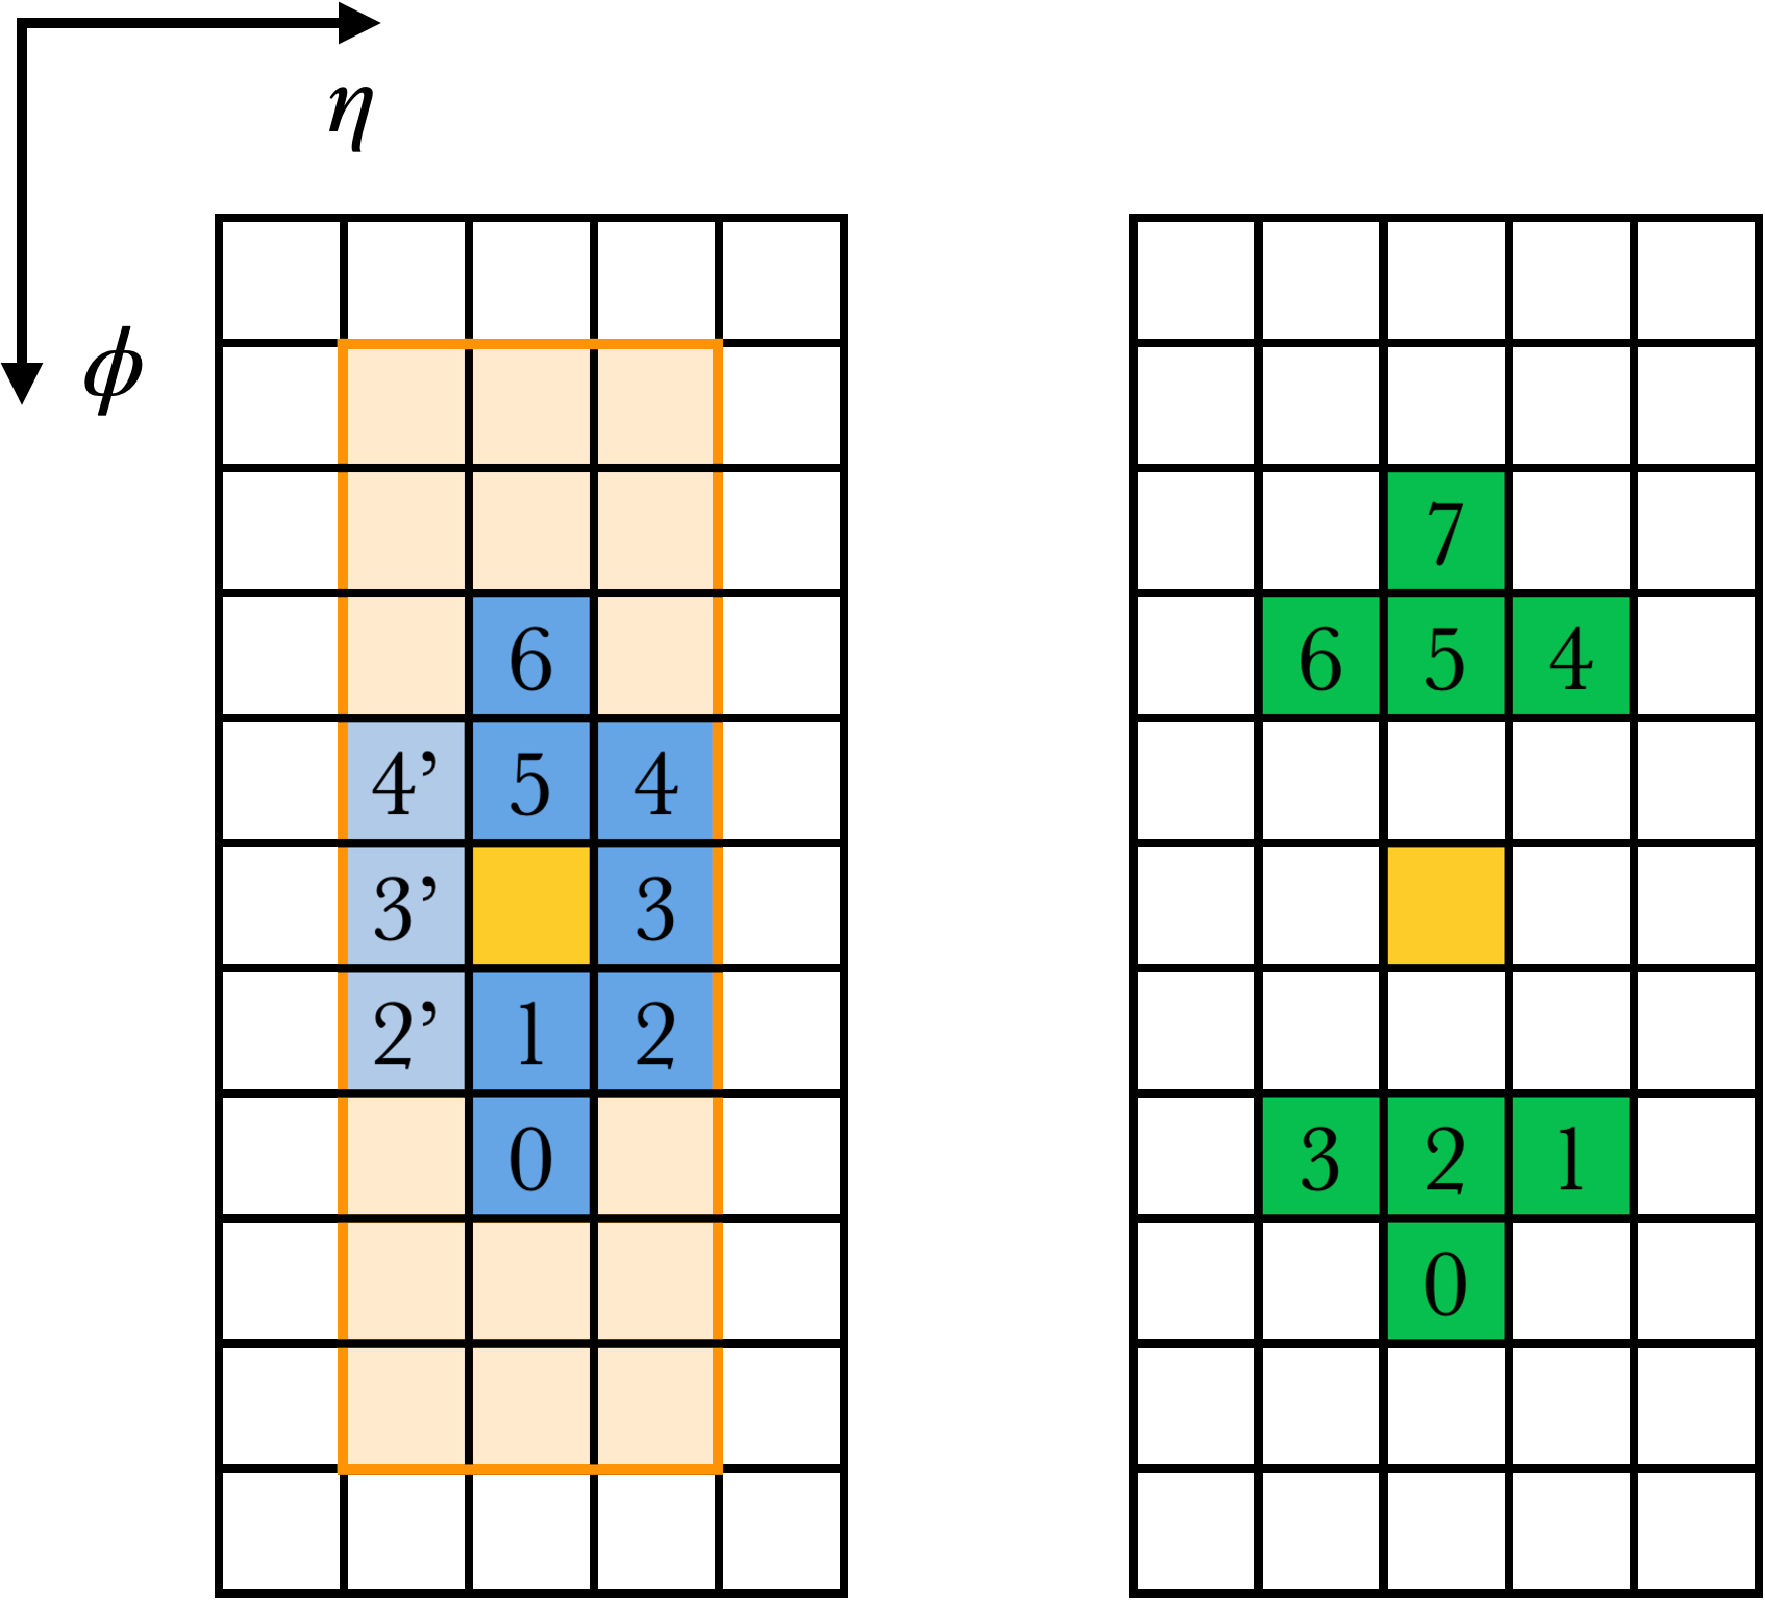
\includegraphics[width=0.4\linewidth]{Figures/L1TP/L1TauCluster.pdf}
    \caption{Schematic for the $\tau_h$ dynamic clustering algorithm. A candidate is initiated by the definition of a proto-clustering, consequently trimmed to remove the least energetic side (left). Additional secondary clusters can be merged to the primary one, if their seed lies within the seven green TTs (right); the secondary clusters seeded in position 2 or 5 are not considered if their seed is already included in the primary proto-cluster.}
    \label{fig:L1TauCluster}
\end{figure}

\subsubsection{Jet candidates}

The hadronic jet candidates are defined from a fixed dimension clustering approach. 
The L1 jet candidate is initiated by the presence of a high energy deposit in a single TT seed, and the surrounding matrix of $9\times9$ TTs defines as the jet cluster. 
The size of the window is chosen to correspond to the $\Delta R = 0.4$ angular opening, which is radius used for the offline anti-$k_T$ reconstruction algorithm~\cite{Zabi_2016}.
In order to avoid double counting of jets, a jet candidate is discarded if any of the TTs composing the cluster has an energy deposit greater than the central seed.
The energy in the $9\times9$ cluster, also known as \textit{chunky donut}, is defined to be the raw jet energy.

Given the large extension of the jet candidate, a dedicate pile-up subtraction method is implemented, which estimates the energy deposit due to pile-up and subtracts it to the jet raw energy deposit.
Two techniques for local pile-up correction are available in the Layer-2 algorithm employed during Run~III data taking:
\begin{itemize}
    \item Chunky donut subtraction: the pile-up energy is estimated as the sum of the energy deposit in the four $9\times3$ strips around the chunky donut, removing the highest and lowest energy sides.
    \item Phi-ring subtraction: the pile-up energy is estimated as the energy deposit on 9 rings of TTs with the same $\eta$ coordinates, re-scaling the surface to the $9\times9$ of the jet candidate.
\end{itemize}

As a last step, the Layer-2 jet candidates are calibrated based on their raw energy and $\eta$ position.

\begin{figure}
    \centering
    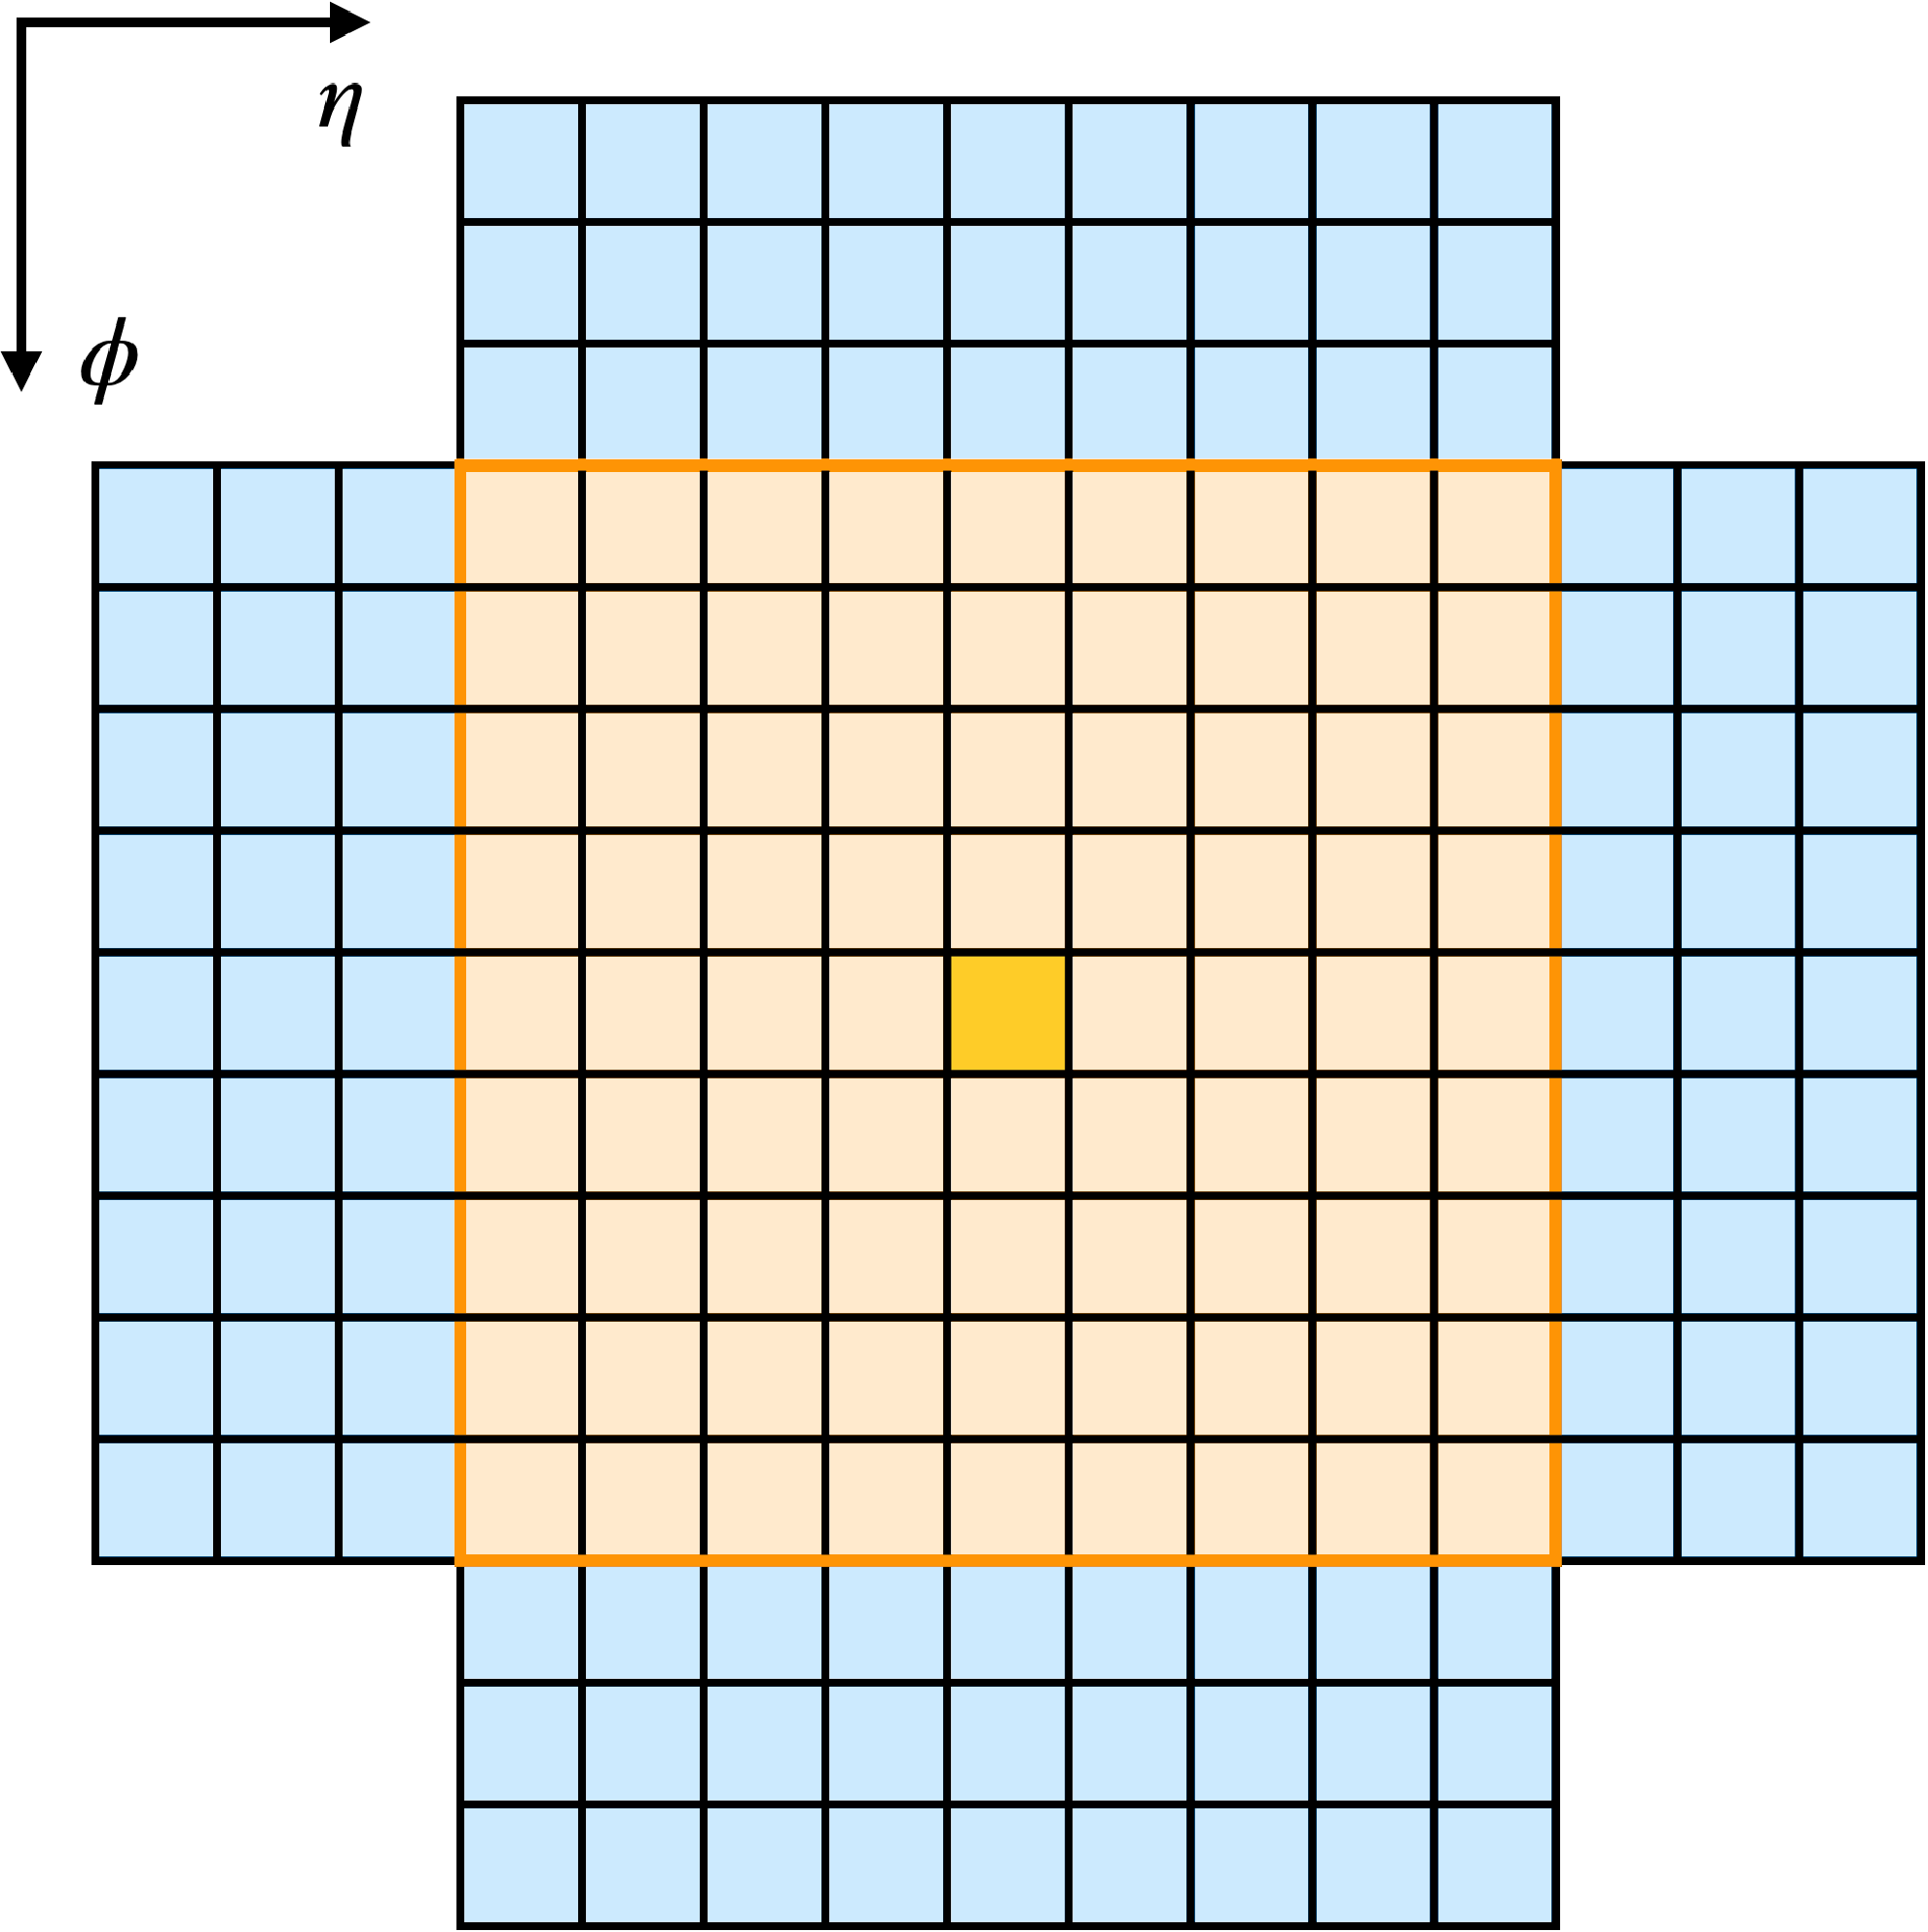
\includegraphics[width=0.4\linewidth]{Figures/L1TP/L1JetCluster.pdf}
    \caption{Schematic for the jet $9\times9$ chunky donut cluster. The four calorimeter strips around the chunky donut are used to estimate the local energy density due to piel-up.}
    \label{fig:L1JetCluster}
\end{figure}

\subsubsection{Energy sums candidates}

The energy sums are the last objects to be constructed in the L1 calorimeter trigger, as they involve full calorimeter granularity.
The total missing transverse energy $E_T^{miss}$ is computed by splitting the regional TTs energies into their $x$ and $y$ components, and summing the components in quadrature.
The resulting vector, after a rotation of $180^{\circ}$, provides the magnituse and angle of the missing energy due to neutrinos not interacting with the detector material.
The total scalar transverse energy of all jets $H_T$ is given by the sum over all clustered jets found in the event.
A dedicated pile-up subtraction and calibration is applied to $E_T^{miss}$ candidate to remove the large contribution coming from soft, diffuse pile-up energy deposits.
The pile-up contribution is estimated from the tower activity in the central part of the barrel and 

\begin{figure}
    \centering
    \subfloat[]{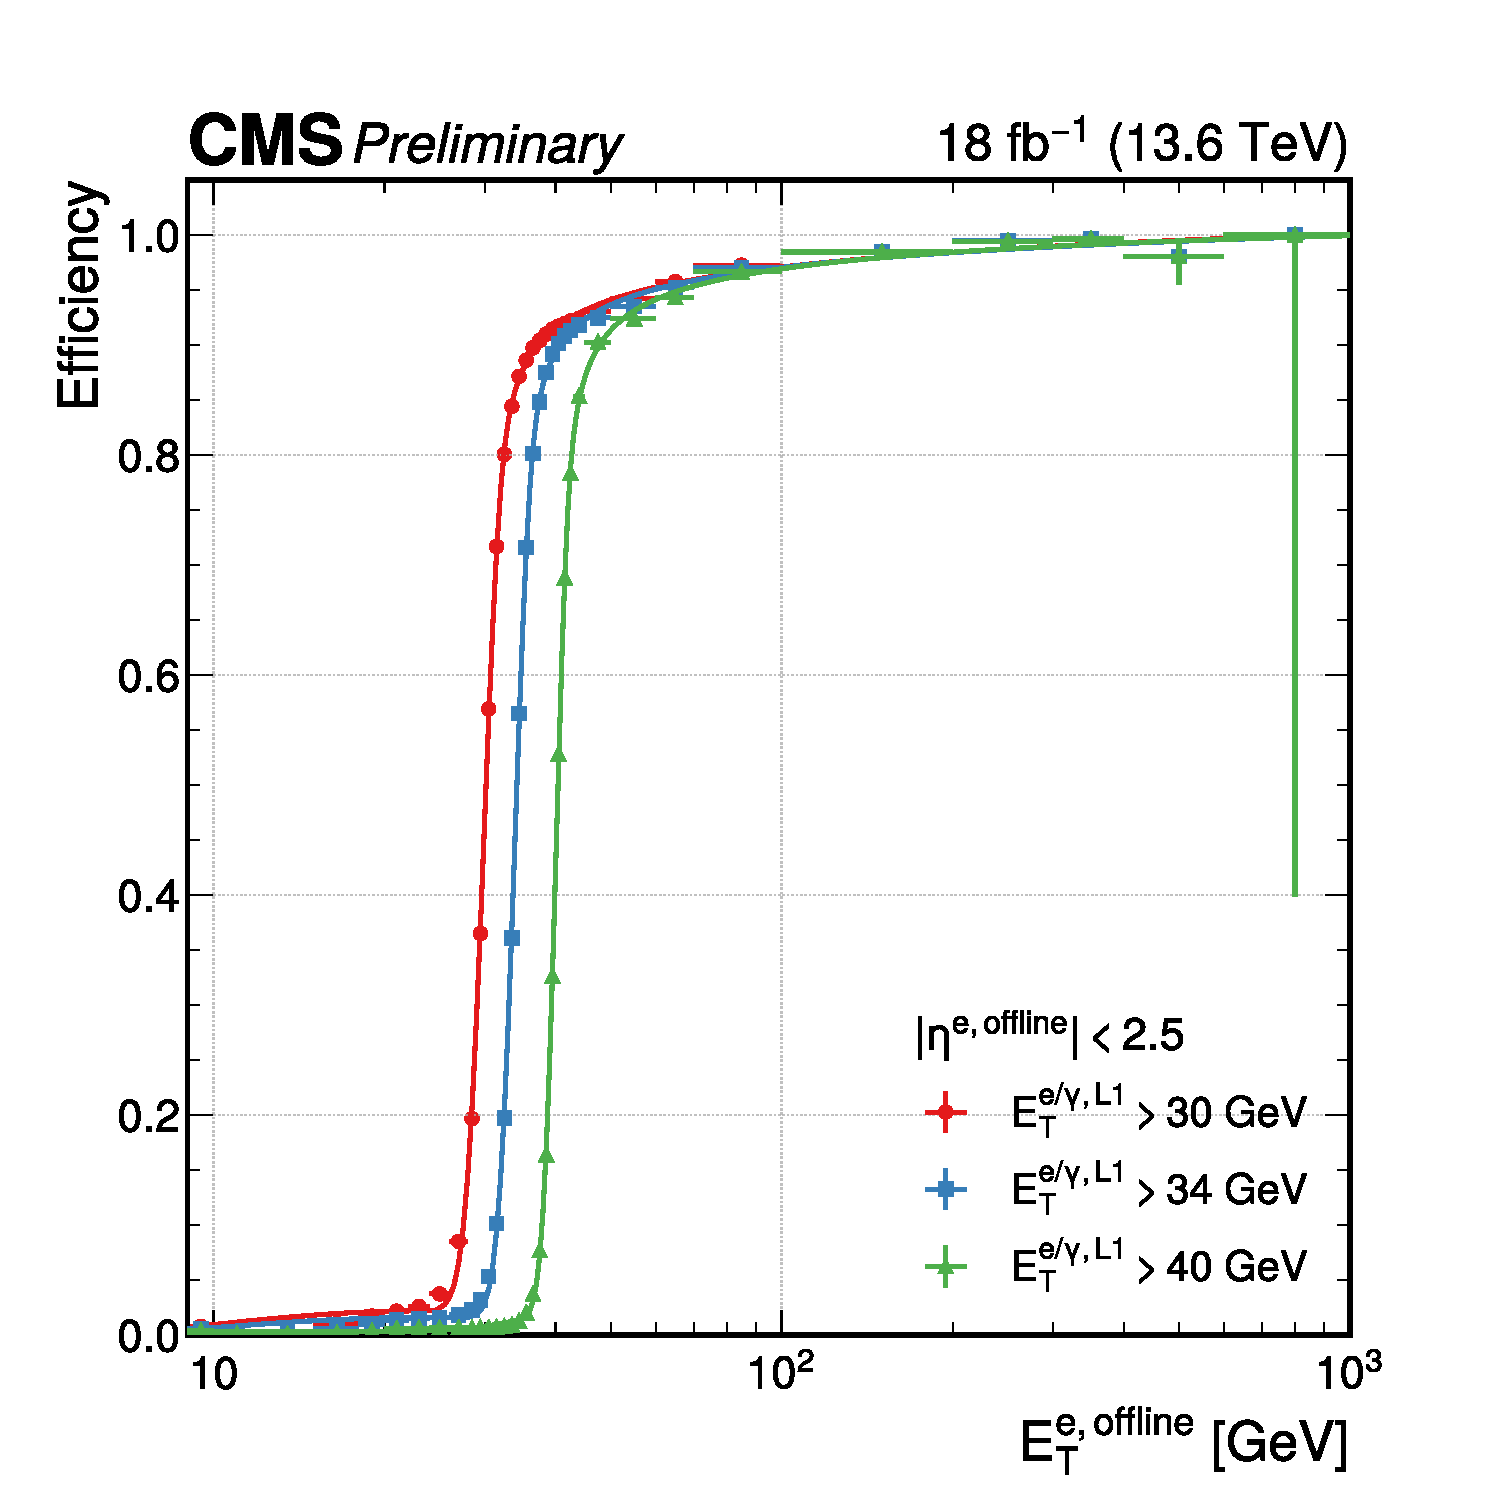
\includegraphics[width=0.4\linewidth]{Figures/L1TP/EGEfficiency.pdf}}
    \subfloat[]{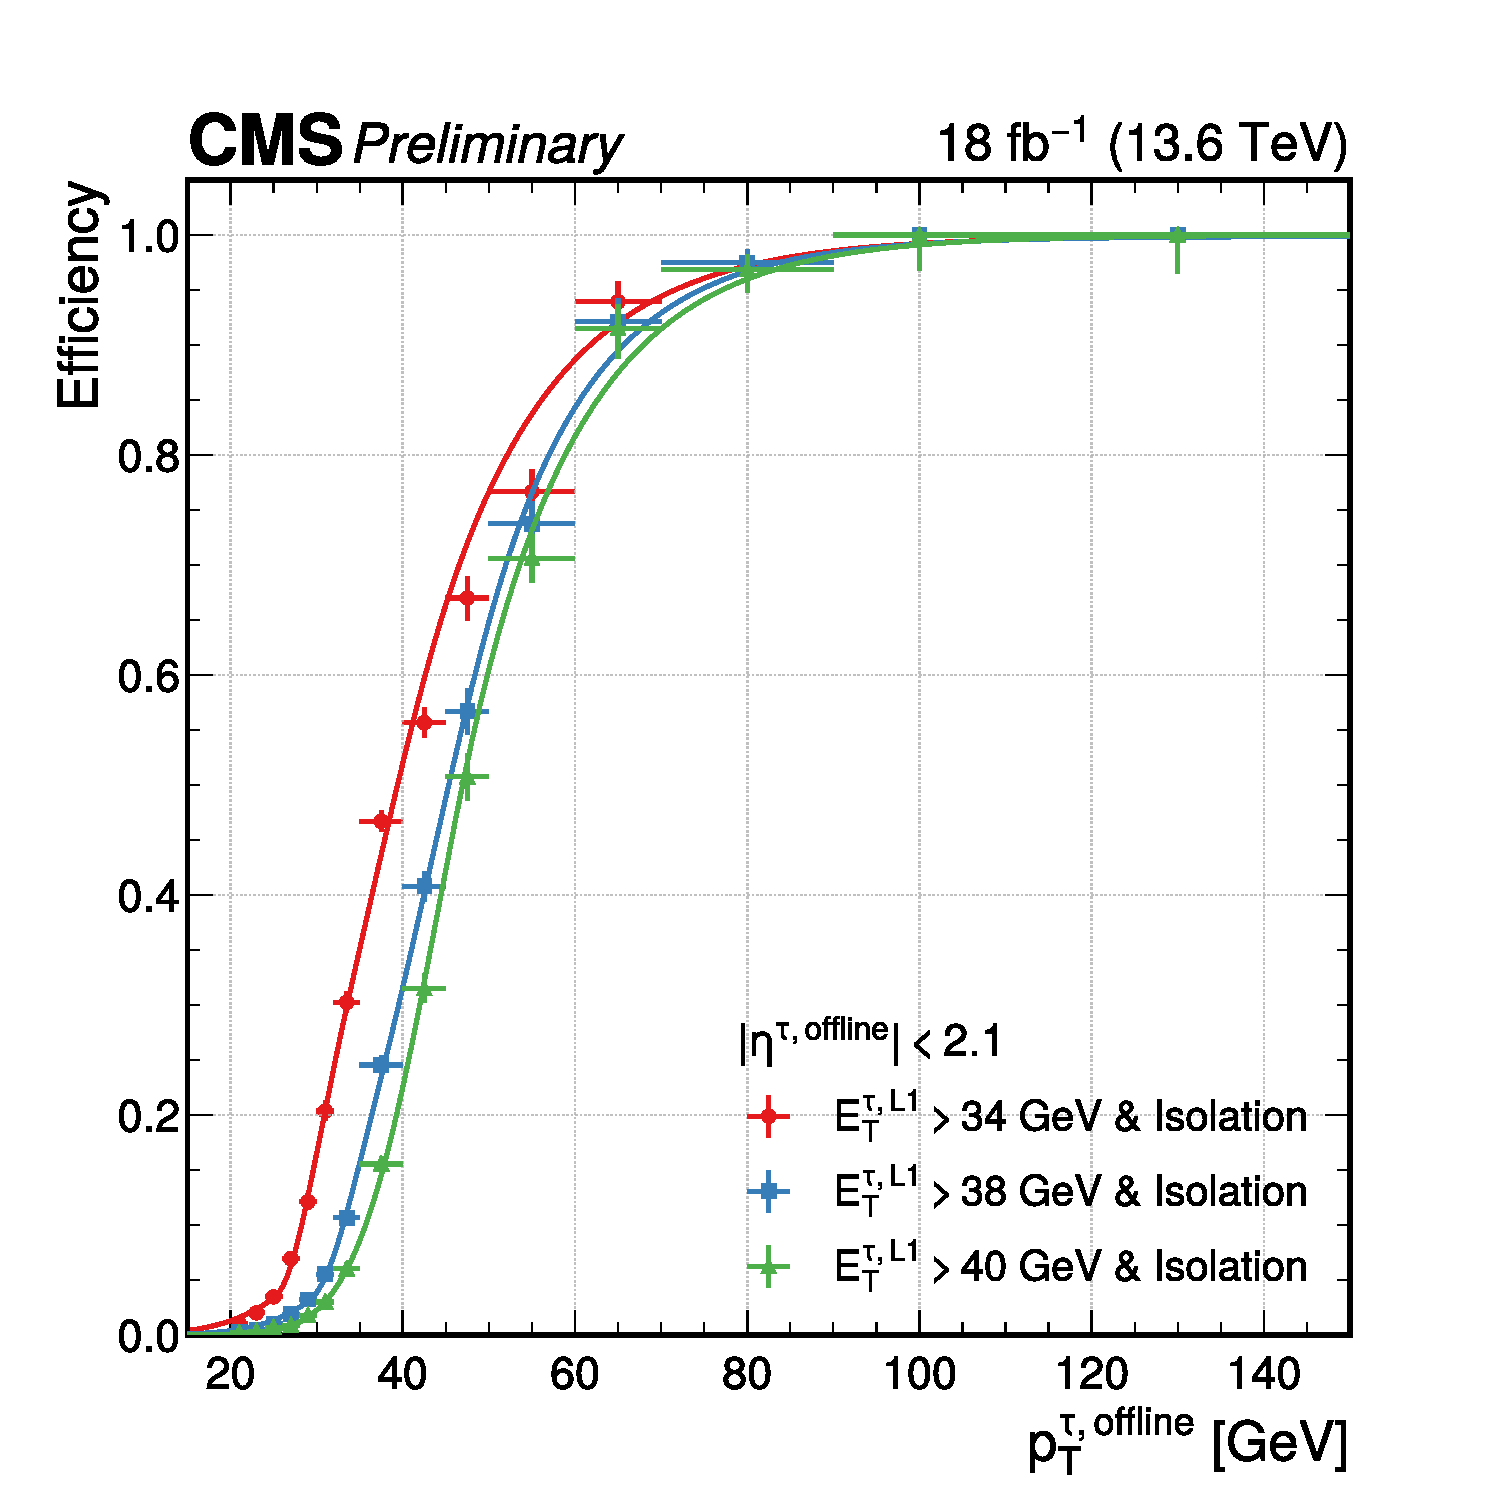
\includegraphics[width=0.4\linewidth]{Figures/L1TP/TauEfficiency.pdf}}
    
    \subfloat[]{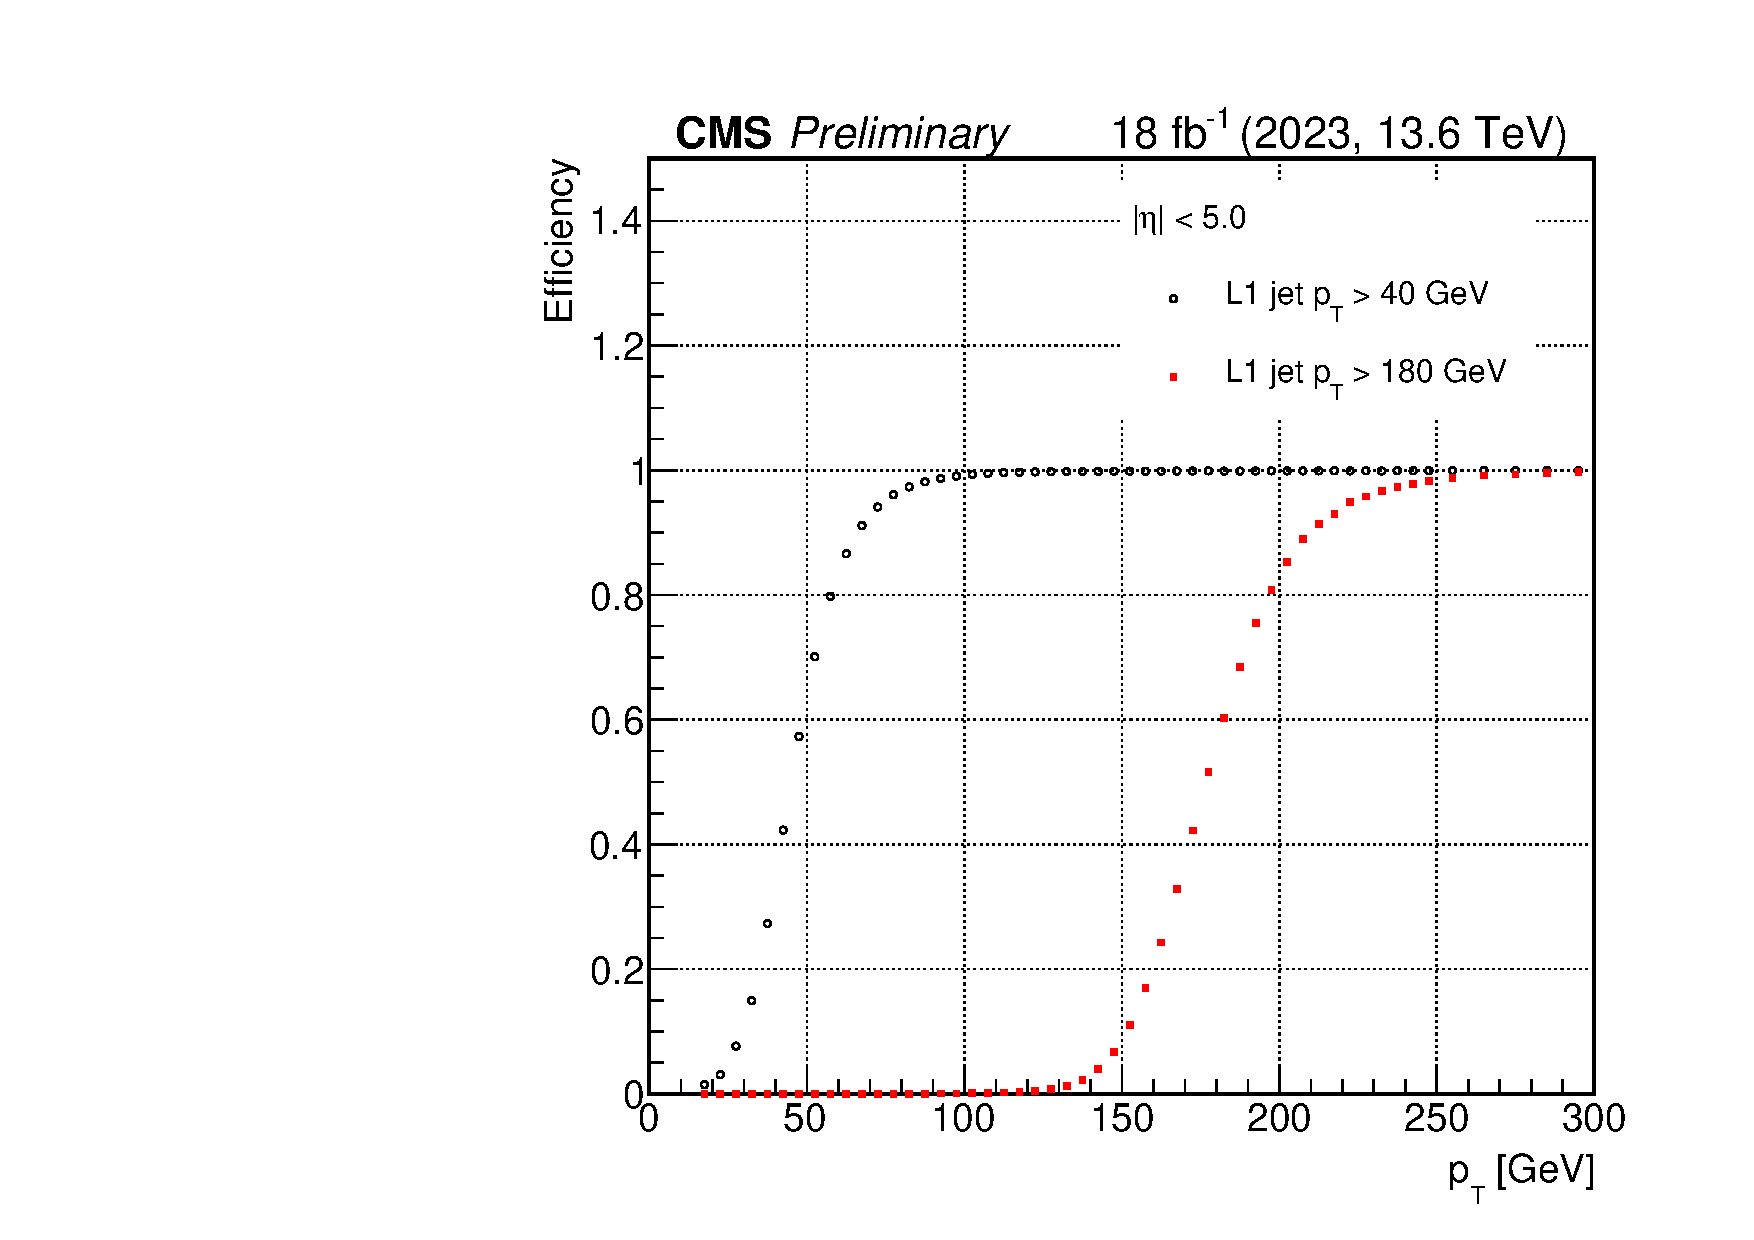
\includegraphics[width=0.4\linewidth]{Figures/L1TP/JetEfficiency.pdf}}
    \subfloat[]{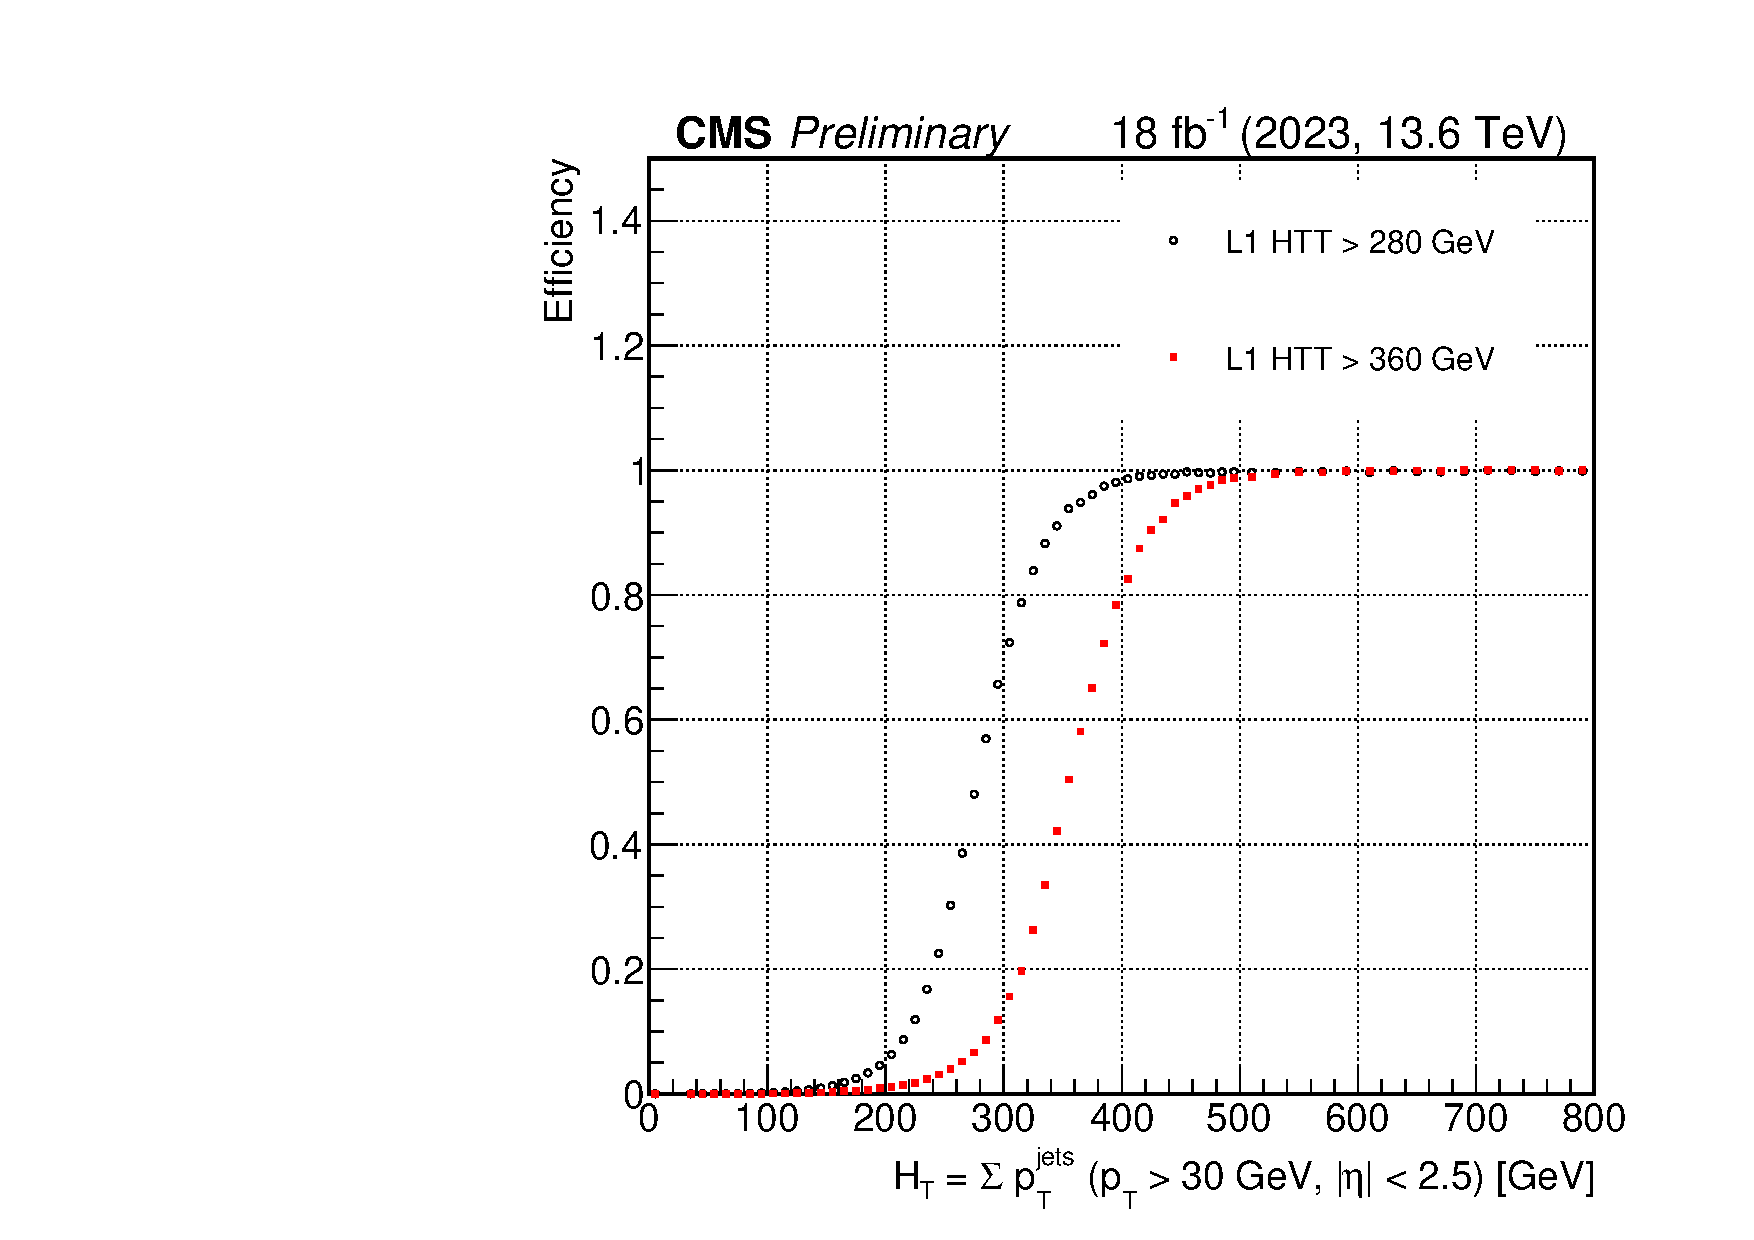
\includegraphics[width=0.4\linewidth]{Figures/L1TP/HTTEfficiency.pdf}}
    \caption{Level-1 performance of L1 calorimeter trigger objects: $e/\gamma$ (a), $\tau_h$ (b), jet (c), and $H_T$ (d). The efficiency turn-on curves are reported for different L1 $p_T$ thresholds.}
    \label{fig:L1Efficiency}
\end{figure}

\bigbreak

The performance of the L1 calorimeter trigger in finding the objects candidate and computing their energy is summarised in Figure~\ref{fig:L1Efficiency}, in terms of efficiency turn-on curves.
The reader will understand, at this point, the considerable importance of Layer-1 calibration in building the L1 calorimeter trigger candidates. 
Given the stacked architecture of Layer-1 and Layer-2, where the latter is fully dependent of the former's output, a better calibration of the TPs at Layer-1 can be crucial in improving the Layer-2 performance.

\section{The current Layer-1 calibration}
\label{sec:The current Layer-1 calibration}

A first method to extract Layer-1 calibration factors was developed at the beginning of Run~II. 
The approach relies on the extraction of firmware-compatible calibration factors to be applied to the ECAL and HCAL TPs arriving in the Layer-1 calorimeter trigger from the ECAL and HCAL read-out electronics.
The Layer-1 firmware supports a single calibration constant to be applied to each TP, depending on its $i\eta$ position and recorded raw energy.
In this method, the calibration factors are derived in exclusive regions of energy deposit and $i\eta$ position, by comparing the Layer-1 TT response from MC samples to the energy of generated objects~\cite{Sirunyan_2020}.

The ECAL TPs calibration factors are based on MC simulated events of single photon production in the ideal environment of no pile-up, with a flatten transverse momentum spectrum for the photon $p_T \in [0,200]$~GeV, and flatten $\eta$ distribution.
For each event, the generated photons are matched to the corresponding TP, based on the ($\eta$, $\phi$) position, which will be considered as the seed. The $e/\gamma$ candidate is approximated as the $3\times3$ cluster centered around the seed. 
Only clusters containing at least 90\% of the total energy in the central tower are considered for the calibration procedure.
The energy binning is defined according to the energy of the central TP, with a pre-defined binning $E_T\in[0,3,6,9,12,15,20,25,30,35,40,45,55,70,127.5]$~GeV.
The clusters are further divided into 28 bins according to the absolute $i\eta$ position of the central TP, i.e. $|i\eta|\leq28$.
In each ($E_T$, $i\eta$) bin, the differential distribution of the uncalibrated Layer-1 response, defined as the ratio between the generated photon transverse momentum and the $3\time3$ cluster energy deposit $p_T^{\gamma}/E_T^{3\times3}$, is interpolated with a Landau distribution convoluted with a Gaussian distribution.

The HCAL TPs calibration factors are obtained following the same procedure detailed above the ECAL, using a MC sample of double charged pion production in the ideal environment of no pile-up; the pions are characterised by a flatten transverse momentum spectrum $p_T\in[0,200]$~GeV and flatten $\eta$ distribution.
Since objects tend to deposit energy in ECAL before reaching HCAL, the HCAL calibration factors are derived considering ECAL TPs in their derivation, and applying the previously extracted ECAL Layer-1 calibration.
For each event, the generated pions are matched to the corresponding TP, based on the ($\eta$, $\phi$) position, and a window of $5\times5$ in ECAL and HCAL centered around the seeding TP is considered as the jet cluster candidate.
It should be noted that in this method the jet cluster size is significantly reduced with respect to the $9\times9$ chunky donut actually used in the Layer-2 algorithm.
Only clusters containing at least 20\% of the total energy in the central tower are considered for the calibration procedure.
The events are binned according to the energy of the central TP, with the same pre-defined binning as ECAL, and to its absolute $i\eta$ position, i.e. $|i\eta|\leq41 \setminus \{29\}$.
For the HF calibration factors, the ECAL contribution is not considered, as the ECAL detector is not present in that pseudorapidity region.
In both cases, saturated towers with energy $E_T=127.5$~GeV are ignored by the calibration procedure. 

The calibration factors are originally designed to be extracted by the mean of the fitted distribution; however, given the presence of large tails towards higher energies, the method has been upgraded in 2018 to use the mode, i.e. the value that appears most frequently in the distribution.
An example for the interpolation of the response distributions is reported in Figure~\ref{fig:OldL1Fit}, for ECAL $E_T \in [0,3]$~GeV and $i\eta=1$~(a), and for HF $E_T \in [0,3]$~GeV and $i\eta=31$~(b).

The extracted calibration constants are stored in three firmware-compatible Look-Up-Tables (LUT), for ECAL, HCAL, and HF respectively. In total, for 13 energy bins and 40 pseudorapidity rings, 520 scale factors are defined, and encoded into 10-bit digital variables.
The resulting values are summarised in Figure~\ref{fig:L1OldSF} for ECAL and HCAL TPs, as a function of $i\eta$ and $E_T$.
The increase of the calibration factors with $\eta$ reflects the profile of the detector material in front of the calorimeters. The choice of the binning respects the hardware limitation and takes into account the dependency of the resolution in $E_T$.

\begin{figure}
    \centering
    \subfloat[]{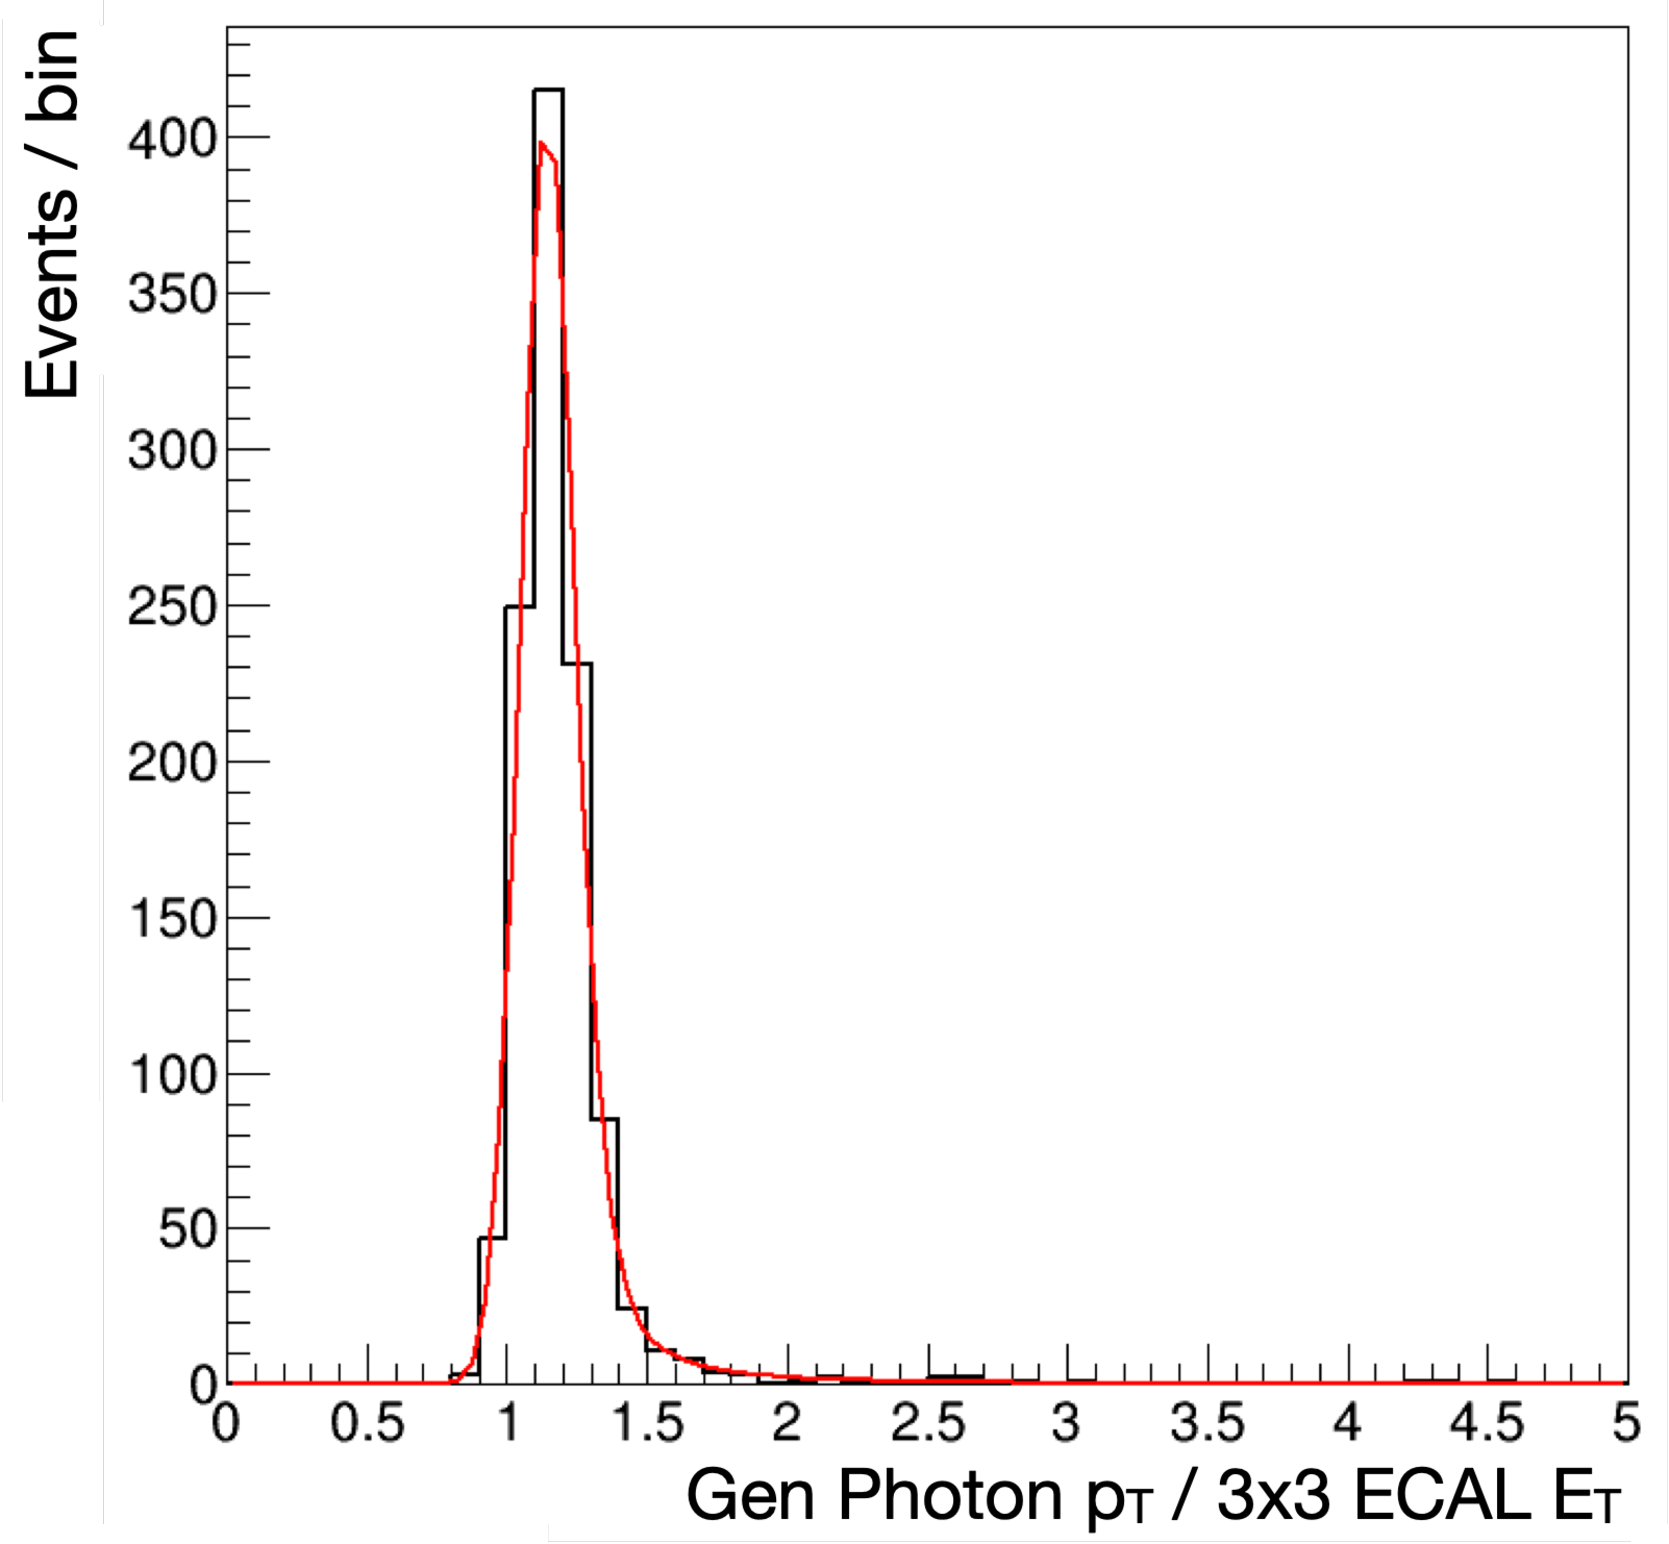
\includegraphics[width=0.4\linewidth]{Figures/L1TP/OldL1ECAL.pdf}}
    \hspace{0.7cm}
    \subfloat[]{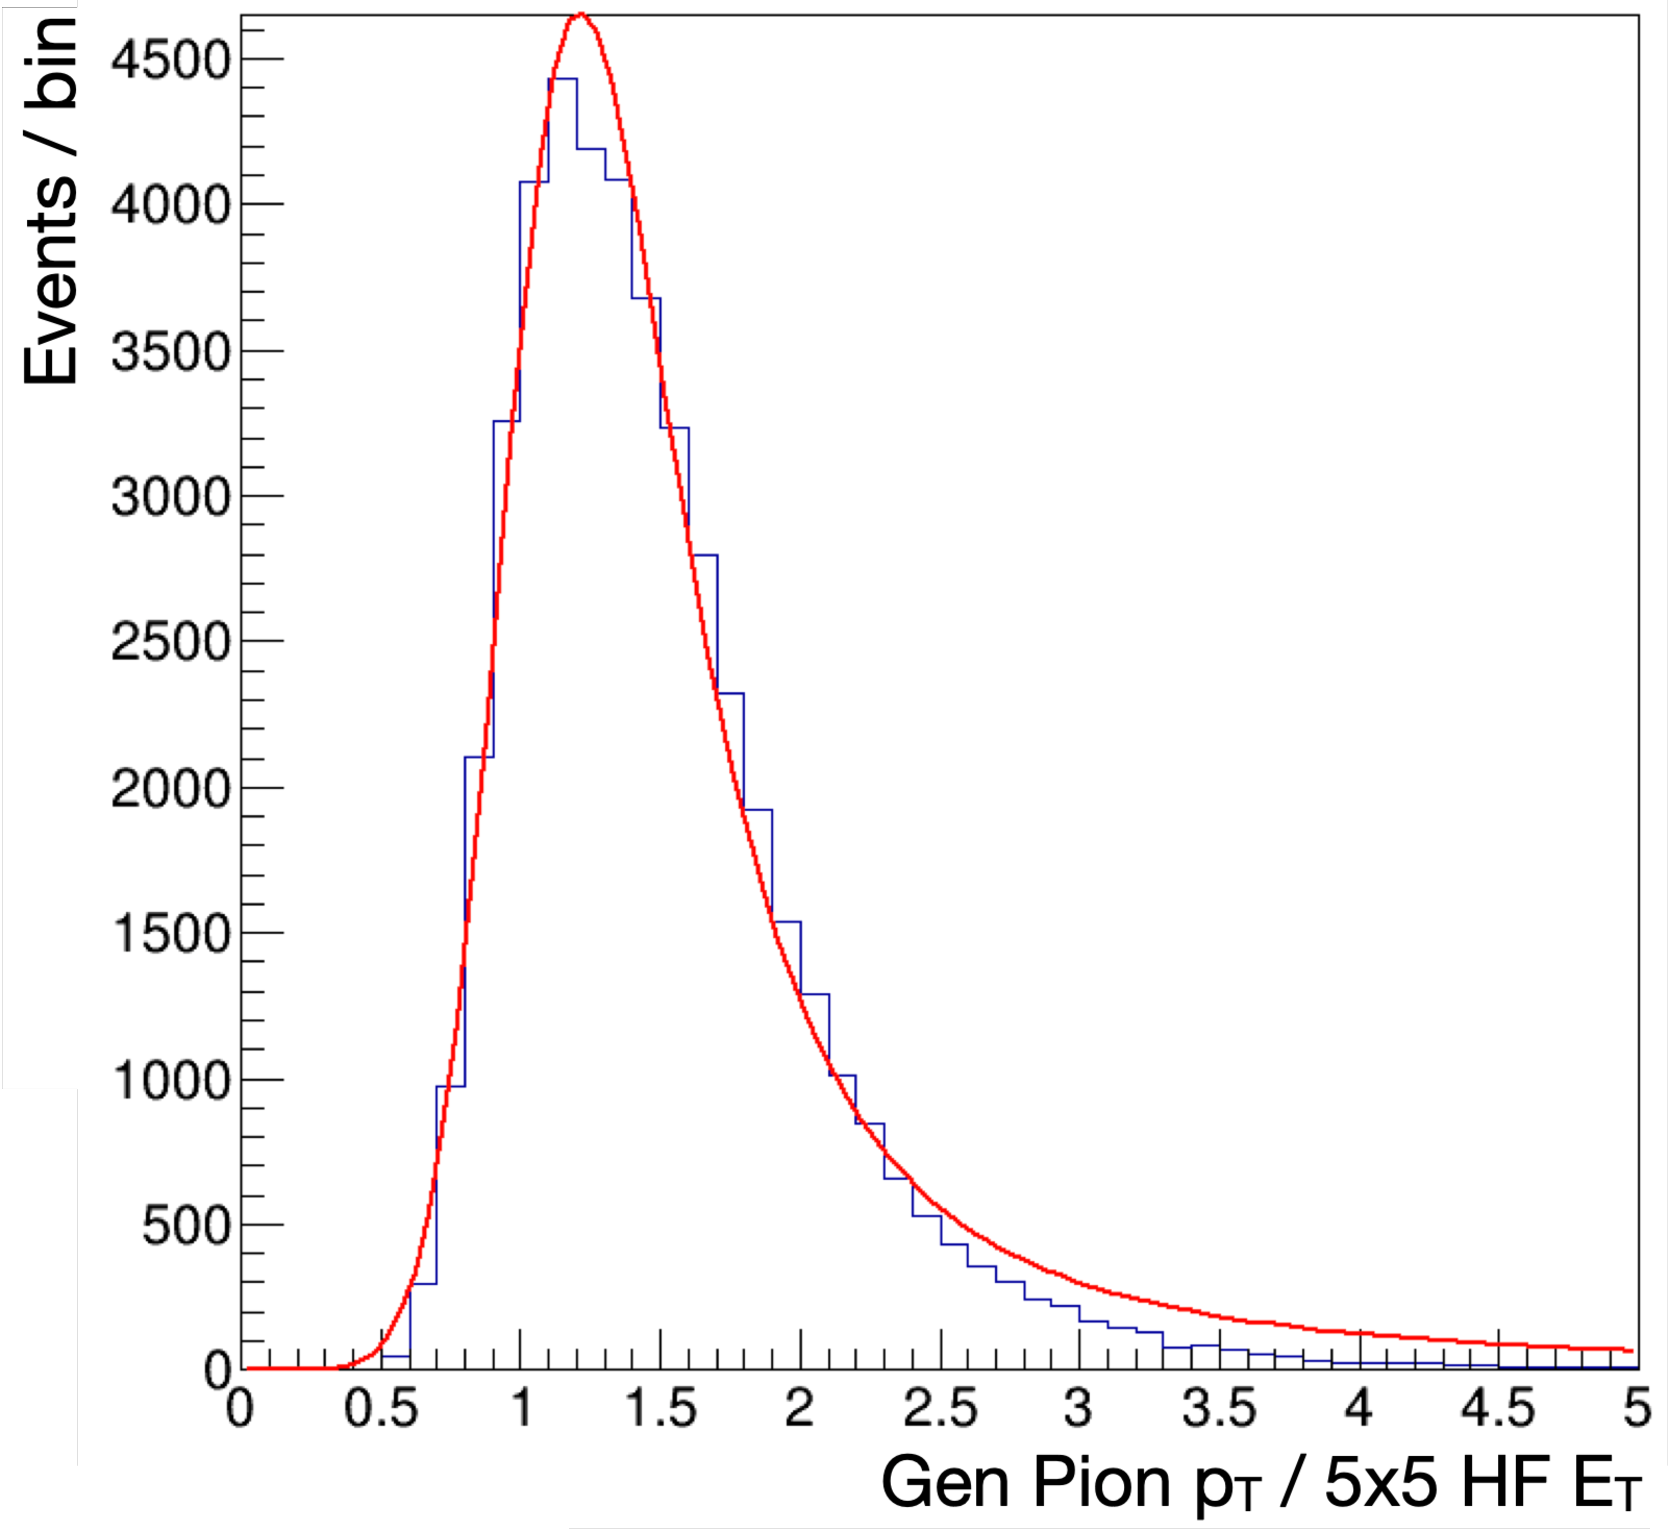
\includegraphics[width=0.4\linewidth]{Figures/L1TP/OldL1HF.pdf}}
    \caption{Distribution of the Layer-1 energy response fitted with a Landau distribution function convoluted with a Gaussian. For ECAL, the response is defined as the ratio between the generated photon transverse momentum and the $3\time3$ $e/\gamma$ cluster energy deposit for $E_T \in [0,3]$~GeV and $i\eta=1$~(a). For HCAL and HF, the response is defined as the ratio between the generated pion transverse momentum and the $5\time5$ jet cluster energy deposit for $E_T \in [0,3]$~GeV and $i\eta=31$~(b).}
    \label{fig:OldL1Fit}
\end{figure}

\begin{figure}
    \centering
    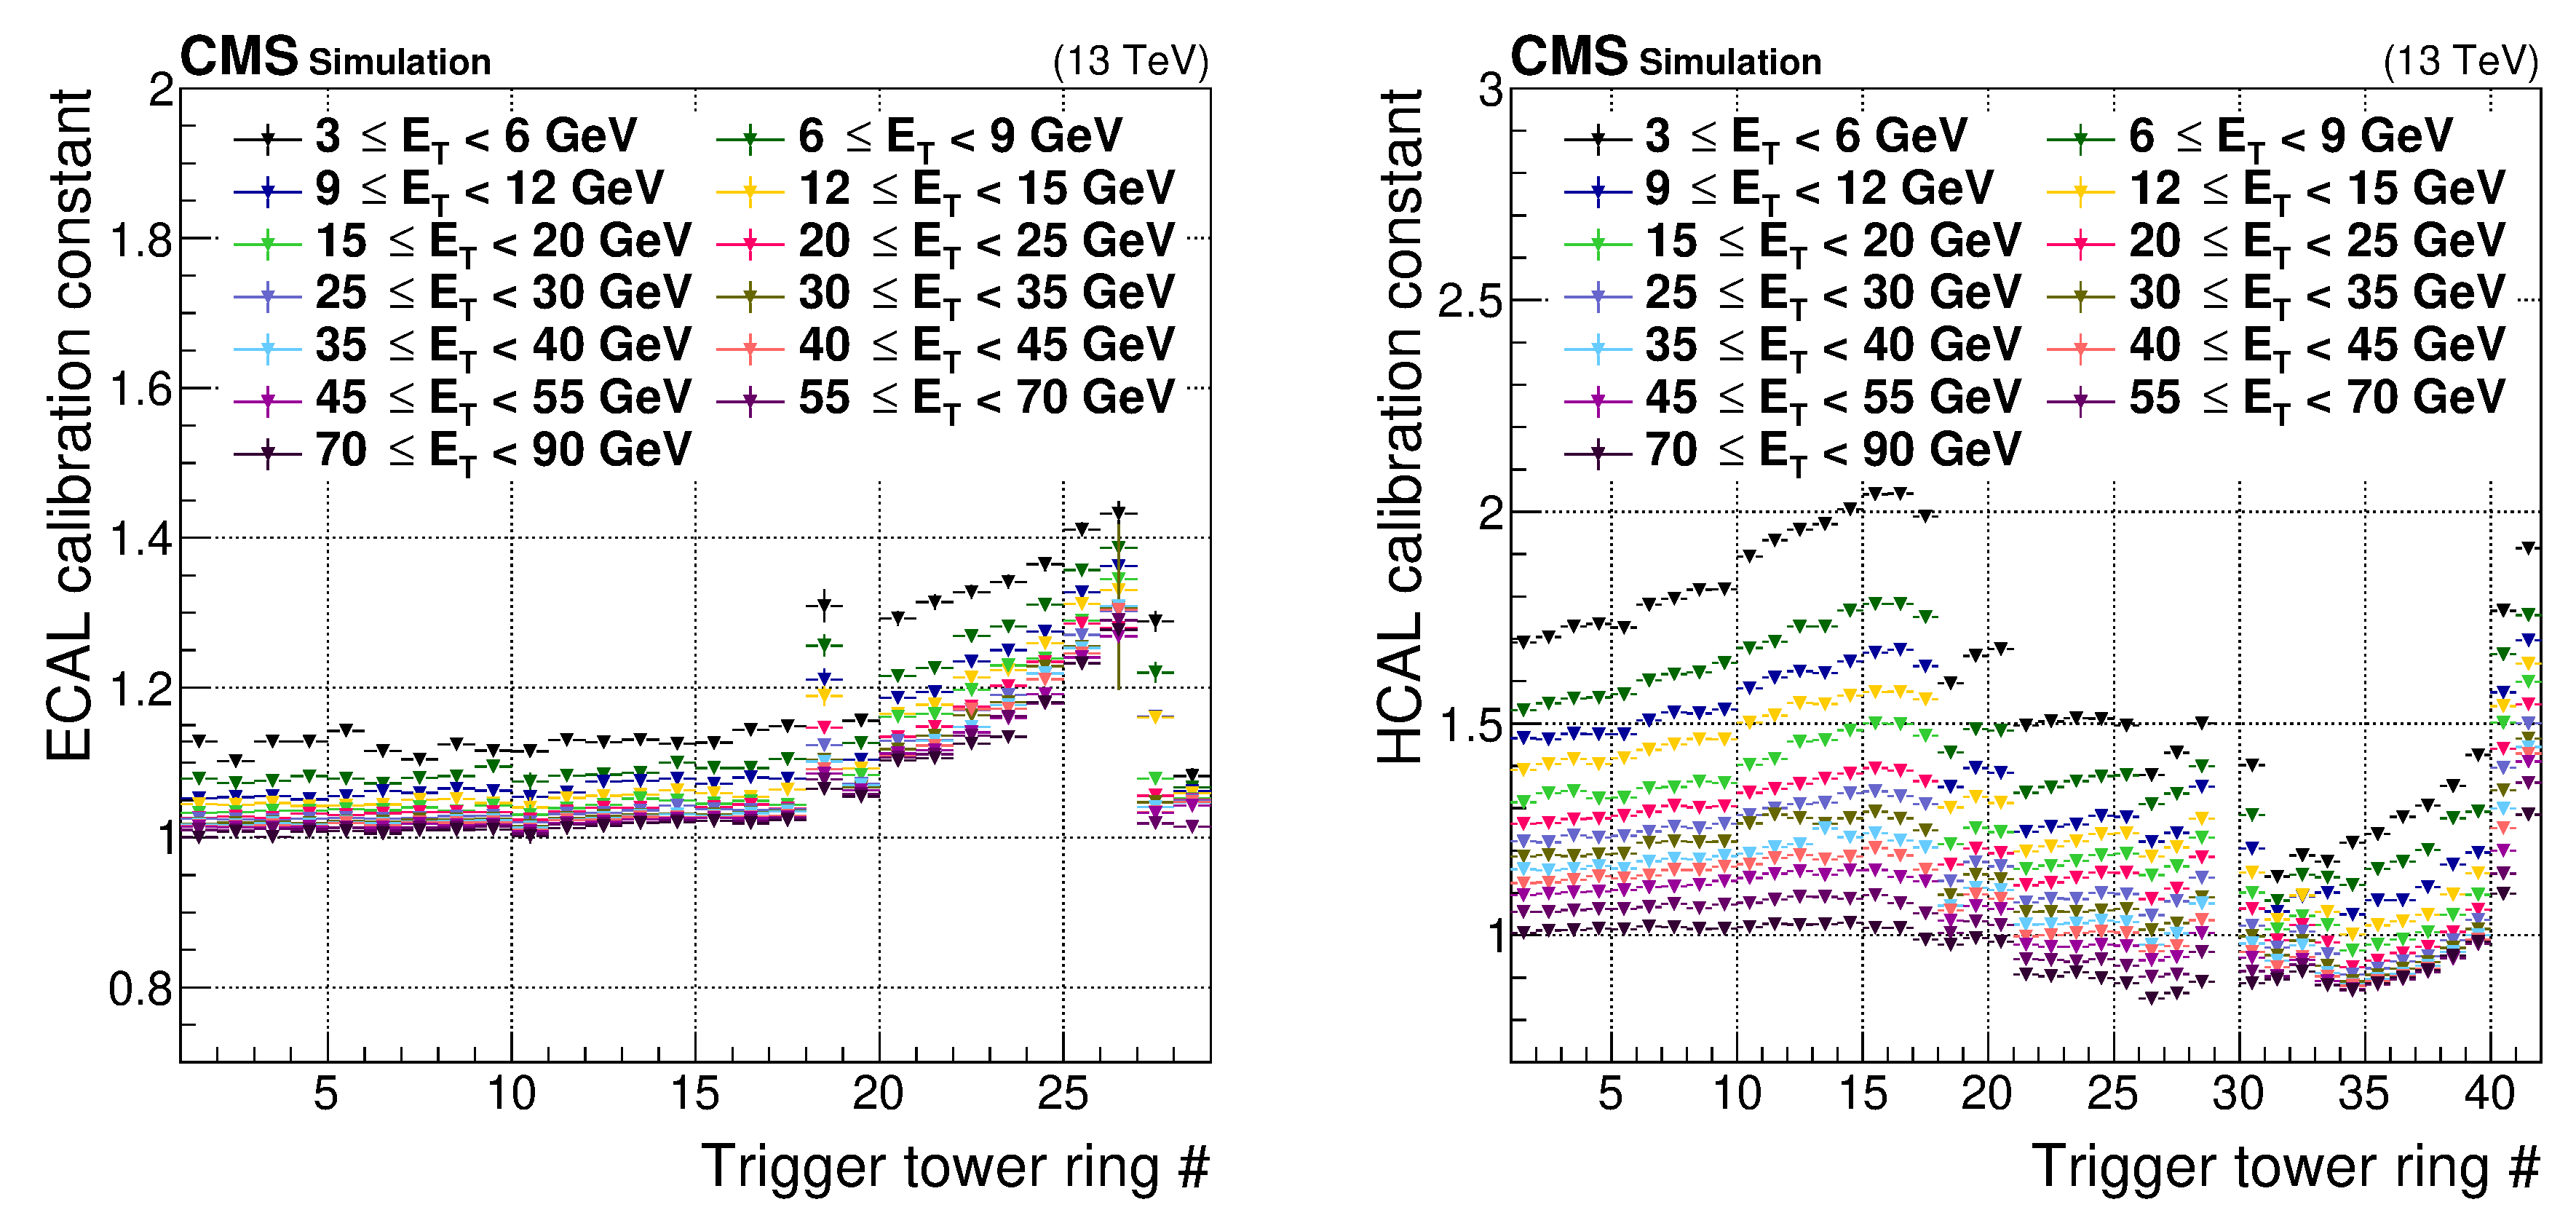
\includegraphics[width=0.9\linewidth]{Figures/L1TP/L1OldSF.pdf}
    \caption{Layer-1 energy scale factors for ECAL (left) and HCAL (right), shown for each constant-$|\eta|$ ring of Trigger Primitives (TP). As specified in the legend, the color of each point corresponds to a range of uncalibrated TP transverse energy values received by the Layer-1 calorimeter trigger. Because of the HCAL geometry, the signals from TPs ring 29 are divided between rings 28 and 30, and no scale factors are applied.}
    \label{fig:L1OldSF}
\end{figure}

\bigbreak

The current method for the extraction of Layer-1 calibration factors has achieved good results throughout Run-II, but suffers from inherent criticality. 
The method is based on the use of MC simulated samples, with particular conditions in terms of flatten energy and $\eta$ distributions, and is affected by its finite statistical power. 
In order to ensure comparable and sufficient statistics in all bins, the approach requires the definition of a small number of coarse energy bins, while the firmware would allow for a finer binning up to one calibration factor every energy digit, i.e. 0.5~GeV.
Moreover, MC samples are based on the simulation of the detector response to generated particles and the simulation of the response in low energy TPs have proven to be not entirely reliable and highly dependent on the continuously varying detector conditions.
Another critical point comes from the definition of the $e/\gamma$ and jet cluster candidates, which does not follow the same algorithm employed in Layer-2; in particular, the HCAL shower can spread beyond the $5\times5$ extension of the cluster.
In addition, once the cluster of multiple TPs has been defined, the calibration factor is only extracted for the central TP through a linear regression. This approach completely ignores any possible dependency on the energy distribution within the cluster or any correlation between different TPs.

These points have become particularly evident at the start of the Run~III data-taking. 
The optimization of ECAL, HCAL, and HF calibrations was performed, but in the case of HCAL and HF, the new correction factors did not pass the necessary validation and closure tests. 
For this reason, for the Run~III data-taking, the choice was made to set HCAL and HF Layer-1 calibration factors to unity, thus removing the needed calibration.

\section{The new Layer-1 calibration}

A novel ML technique for the detector calibration has been developed for the extraction of Layer-1 calibration factors, with the goal of providing a first proof of concept of the ML-based calibration method in a field that is essential for the L1 Trigger system and could have large impact on the entire CMS detector performance.
The ML-based approach aims to resolve some of the critical points coming from the current calibration technique mentioned in the previous section.

The first improvement comes from a redefinition of the clusters defining the $e/\gamma$ and jet candidates. 
According to the Layer-2 conventions for the hadronic jet candidates, the L1 cluster is defined, both for $e/\gamma$ and jet objects, as the $9\times9$ matrix of TTs composing the \textit{chunky donut} (CD). This choice ensures maximal containment of the hadronic shower, and minimal energy loss. This inclusive definition of the L1 cluster has revealed itself as a convenient approach for the calibration of jets, whilst the $e/\gamma$ cluster, initially defined as the same $9\times9$ TTs CD shape, has been subsequently revised to a smaller shape, in order to reduce the contamination from pile-up. 
Moreover, in the new method no requirements are applied to the energy deposit in the central TP, allowing for different candidate shapes to enter the calibration process, expanding the effectiveness of the calibration to account for a wider range of possible shapes.

The second improvement originates from the employment of ML-based algorithms to extract the calibration constants, removing the need for the current linear regression. 
The capability of ML methods to consider all inputs inclusively during the training allows for a faster extrapolation of the calibration constants, without necessitating finite coarse energy bins. In principle, ML techniques do not require any categorisation of the input dataset, being able to learn from all data simultaneously and to interpolate the detector response even for objects that were not part of the input dataset. However, in this specific application, the calibration factors are constrained by the firmware compatibility, limiting the size of the energy bin to $\Delta E_T\geq0.5$~GeV.

Finally, the method described in this Chapter is based on the possibility of extracting the calibration factors using either MC simulated events or data. In the first case, the calibration method benefits from a better definition of the true object energy at generator level, and from the simulation of the ideal environment of no pile-up, hardly achievable during ordinary data taking conditions. In the latter, the use of data presents more arduous conditions due to the inevitable contribution of pile-up, however it provides the most reliable representation of the latest detector response, with particular impact especially when considering low energy deposits.

\bigbreak

The first implementation of the new Layer-1 calibration method has been based on a Neural Network (NN) approach, which I contributed in developing and improving. This first attempt is widely discussed in~\cite{Motta:2881939}, and reported in the next Section~\ref{sec:The Neural Network approach}, however it was found to have intrinsic limitations for the specific application of the calibration to the Layer-1 context. 
As part of this Thesis work, I have also converted the NN method into a new algorithm based on differentiable programming, allowing for streamlined parameter optimisation and better integration of the Layer-1 calibration within the Layer-2 interface.

% The Trigger Primitives that used to build the Level-1 Trigger calorimeter objects (electron, photon, tau leptons, jets, etc.) are calibrated using the method described in Ref. \cite{CMS:2020cmk}. It consists in deriving calibration factors for the ECAL and Hadronic Calorimeter (HCAL) from single-photon (single-pions)
% simulations. The calibration factors are extracted, in bins of $\eta$ and transverse energy, from the distribution of the calorimeter response, i.e. the ratio of the true particle energy (a photon or a pion) to the energy of a group of 3 (9) Trigger Primitives.\\

\section{The Neural Network approach}
\label{sec:The Neural Network approach}
\subsection{Architecture}
\subsection{Input processing}
\subsection{Limitations}

\section{The differentiable programming approach}
\subsection{Discrete approach}
\subsection{Input processing}
\subsection{Training optimisation}
\subsection{Performance evaluation}

\section{Future applications}